\chapter{Implémentation et Validation}
\label{chap:Implémentation et Validation}


Ce chapitre décrit l'implémentation du travail réalisé. Il commence par une présentation des technologies utilisées, suivie de captures d'écran illustrant les différentes fonctionnalités développées. Ensuite, les tests effectués sont exposés.
\newpage
\section{Technologies utilisées}
\subsection*{$\bullet$ SAP Commerce (Hybris)}
\begin{center}
    \centering
    
\includegraphics[scale=0.5]{Figures/SAP.jpg}
    \captionof{figure}{Logo de SAP \cite{SAP}}
    \label{fig:processus}
\end{center} 

SAP Commerce (Hybris) est une plateforme de commerce électronique robuste et évolutive, conçue pour gérer efficacement les catalogues de produits, les commandes, les paiements, ainsi que les interactions avec les clients à travers divers canaux tels que le web, les appareils mobiles, et les points de vente physiques. Dans le cadre de ce projet, SAP Commerce a été choisi pour sa capacité à intégrer des outils de suivi des performances et de marketing, offrant ainsi une gestion complète du commerce en ligne et une expérience utilisateur optimale.

\subsection*{$\bullet$ JEE (JSP)}
\begin{center}
    \centering
    
\includegraphics[scale=0.5]{Figures/jee.png}
    \captionof{figure}{Logo de JEE \cite{JEE}}
    \label{fig:processus}
\end{center} 

JEE (JSP) a été utilisé pour développer la partie frontend de la méthode de paiement. En combinant du code Java et HTML, JSP facilite la création de pages web dynamiques permettant l'affichage interactif des informations de paiement et la gestion des transactions utilisateur. Cette technologie a permis de concevoir une interface utilisateur réactive tout en tirant parti de la flexibilité et de la puissance du backend Java pour assurer une gestion efficace des flux de paiement.
\subsection*{$\bullet$ Spring}
\begin{center}
    \centering
    
\includegraphics[scale=0.4]{Figures/spring.png}
    \captionof{figure}{Logo de Spring \cite{spring}}
    \label{fig:processus}
\end{center} 

Spring a été employé pour développer la logique métier associée à la nouvelle méthode de paiement. Il a permis la création de services back-end pour la validation des paiements, l'interaction avec les systèmes de paiement externes, et le traitement des retours d'information. Grâce à son intégration transparente avec SAP Commerce (Hybris), Spring a assuré une séparation claire des responsabilités et une maintenabilité accrue du code, tout en exploitant ses fonctionnalités avancées pour la gestion des transactions et la sécurité.
\subsection*{$\bullet$ SonarQube}
 \begin{center}
    \centering
    
\includegraphics[scale=0.15]{Figures/sonarqube.png}
    \captionof{figure}{Logo de SonarQube \cite{sonarqube}}
    \label{fig:processus}
\end{center} 

SonarQube est un outil d'analyse statique de code permettant de détecter les bugs, les vulnérabilités de sécurité, et d'évaluer la qualité du code source. Dans ce projet, SonarQube a été utilisé pour analyser le code existant et les nouvelles fonctionnalités ajoutées. L'outil a permis de corriger les bugs et les failles de sécurité identifiés, tout en fournissant des recommandations pour améliorer la structure et la lisibilité du code, garantissant ainsi le respect des standards de qualité requis par le client.
\subsection*{$\bullet$ Ant}
\begin{center}
    \centering
    
\includegraphics[scale=0.05]{Figures/Ant.png}
    \captionof{figure}{Logo d'Ant \cite{ant}}
\end{center}

Ant est un outil de build open-source qui permet d'automatiser diverses tâches liées au processus de développement, telles que la compilation, le déploiement, et l'exécution des tests. Dans le cadre de ce projet, Ant a été utilisé pour automatiser la compilation du code, faciliter le débogage, et exécuter les tests unitaires. Grâce à sa configuration native avec Hybris, qui utilise des scripts Ant prédéfinis, Ant a contribué à une organisation efficace des étapes de développement, assurant ainsi un flux de travail structuré et fluide.
\subsection*{$\bullet$ JUnit}
\begin{center}
    \centering
    
\includegraphics[scale=0.5]{Figures/junit.png}
    \captionof{figure}{Logo de JUnit\cite{junit}}
    \label{fig:processus}
\end{center}

JUnit est un framework de tests unitaires en Java utilisé pour tester les composants individuels d'une application. Pour l'intégration de la nouvelle méthode de paiement, JUnit a été employé pour écrire des tests unitaires afin de vérifier la fiabilité des fonctionnalités back-end. Les tests couvraient divers scénarios, y compris la validation des transactions, la gestion des erreurs, et les interactions avec les systèmes externes.
\section{Illustration de l'Intégration de la Méthode de Paiement}
Cette partie fournit une vue détaillée des fonctionnalités développées à travers une série de captures d’écran.
Avant de finaliser l'intégration de Payconiq via Adyen, il est crucial de vérifier que cette méthode de paiement est correctement activée dans le système. Comme le montre la figure \ref{fig:activ}, Payconiq est marqué comme actif dans le Cockpit d'administration de SAP Commerce. 
Cela confirme qu'il est prêt à être utilisé pour le traitement des paiements, garantissant que les transactions effectuées avec Payconiq seront traitées correctement.
\begin{center}
    \centering
    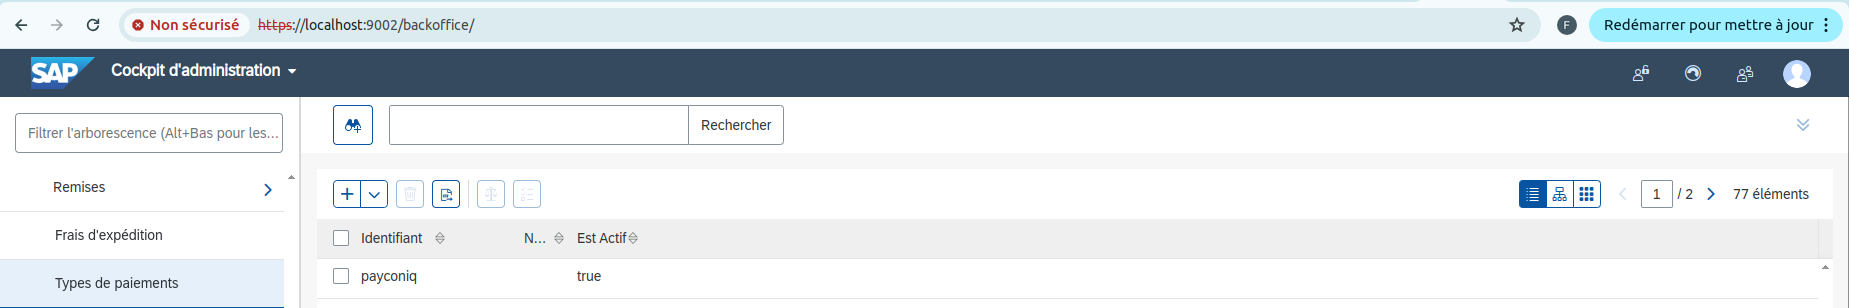
\includegraphics[width=19cm]{Figures/Screens/VERIFIER QUE payment activer.png}
    \captionof{figure}{Activation de Payconiq}
    \label{fig:activ}
\end{center}

Une fois activée, Payconiq a été ajoutée à la boutique en ligne pour le marché belge. La figure \ref{fig:disp} montre que Payconiq apparaît désormais parmi les méthodes de paiement disponibles dans l'onglet eCommerce, aux côtés de giftcard, applepay-eu, et paypal-eu. Cette configuration permet aux utilisateurs de choisir Payconiq lors de la validation de leur commande.
\begin{center}
    \centering
    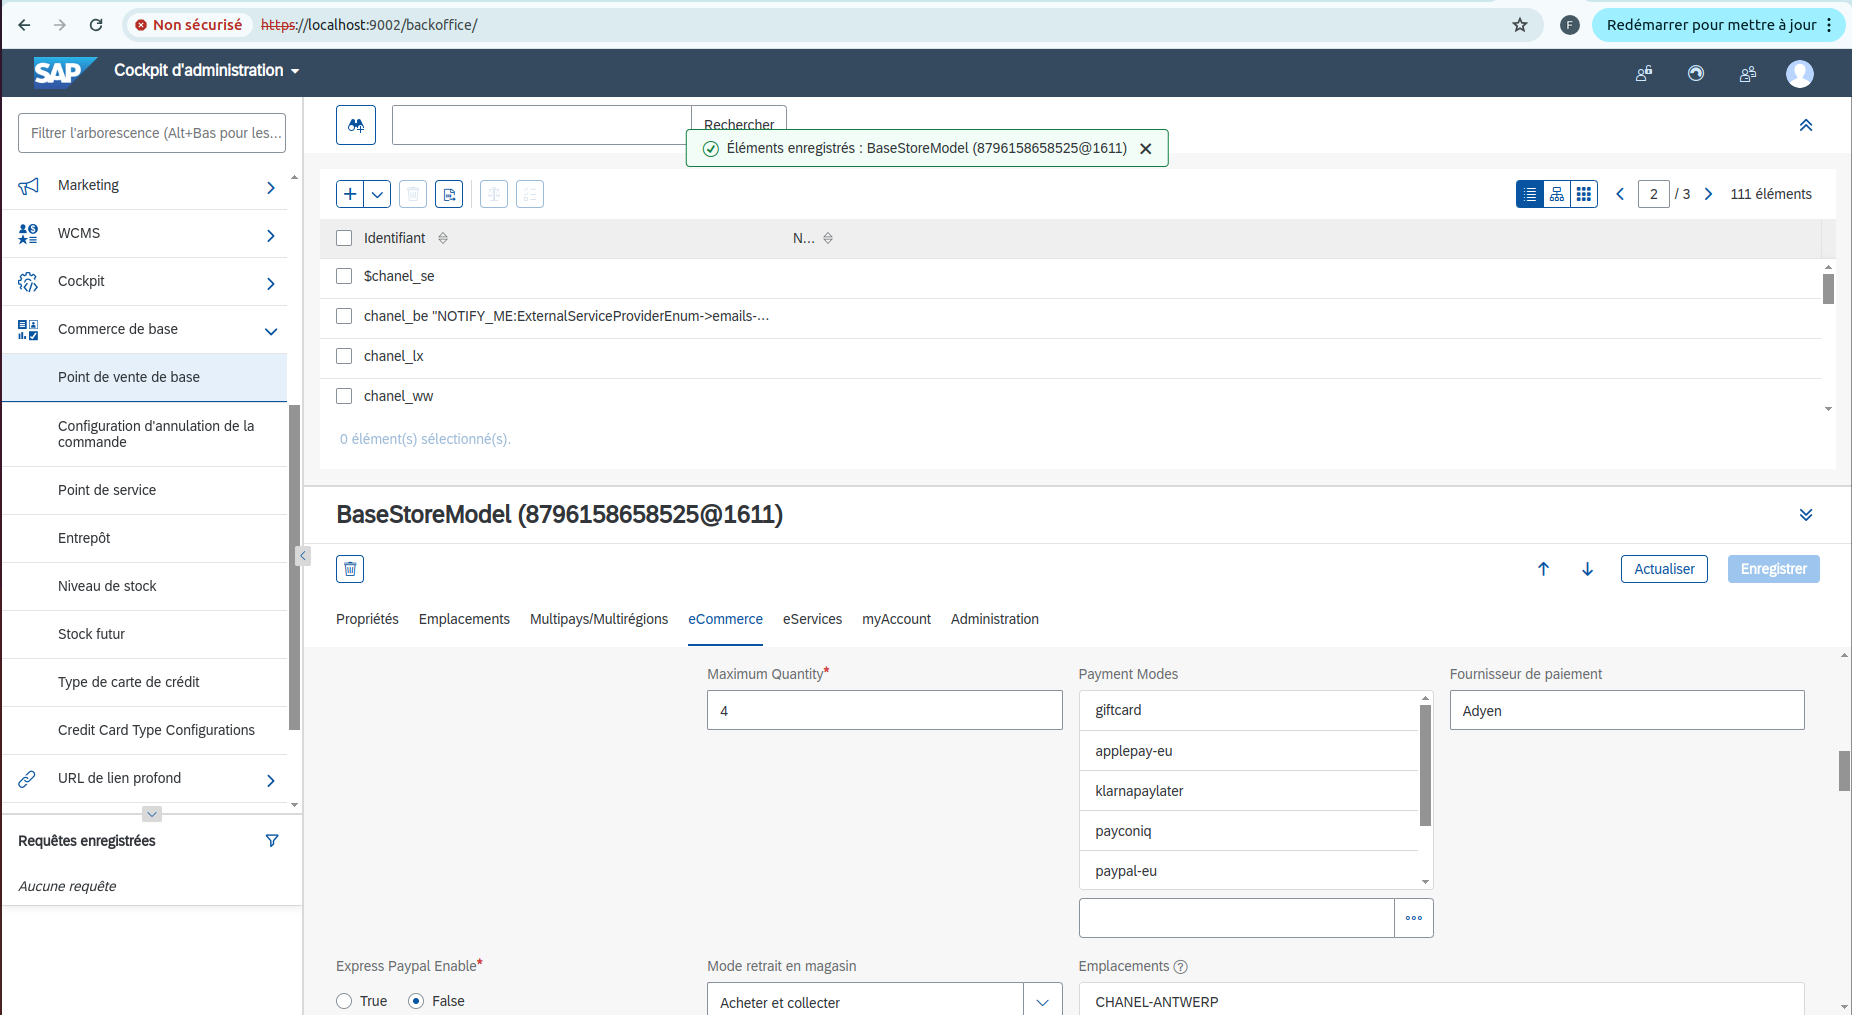
\includegraphics[width=19cm]{Figures/Screens/activation du payconiq pour belge.png}
    \captionof{figure}{Disponibilité de Payconiq dans la boutique en ligne}
    \label{fig:disp}
\end{center}
Lorsque le client sélectionne les articles désirés, il passe à la phase de paiement. La figure \ref{fig:selection} illustre l'ajout d'un produit au panier, une étape préalable au paiement.
\begin{center}
    \centering
    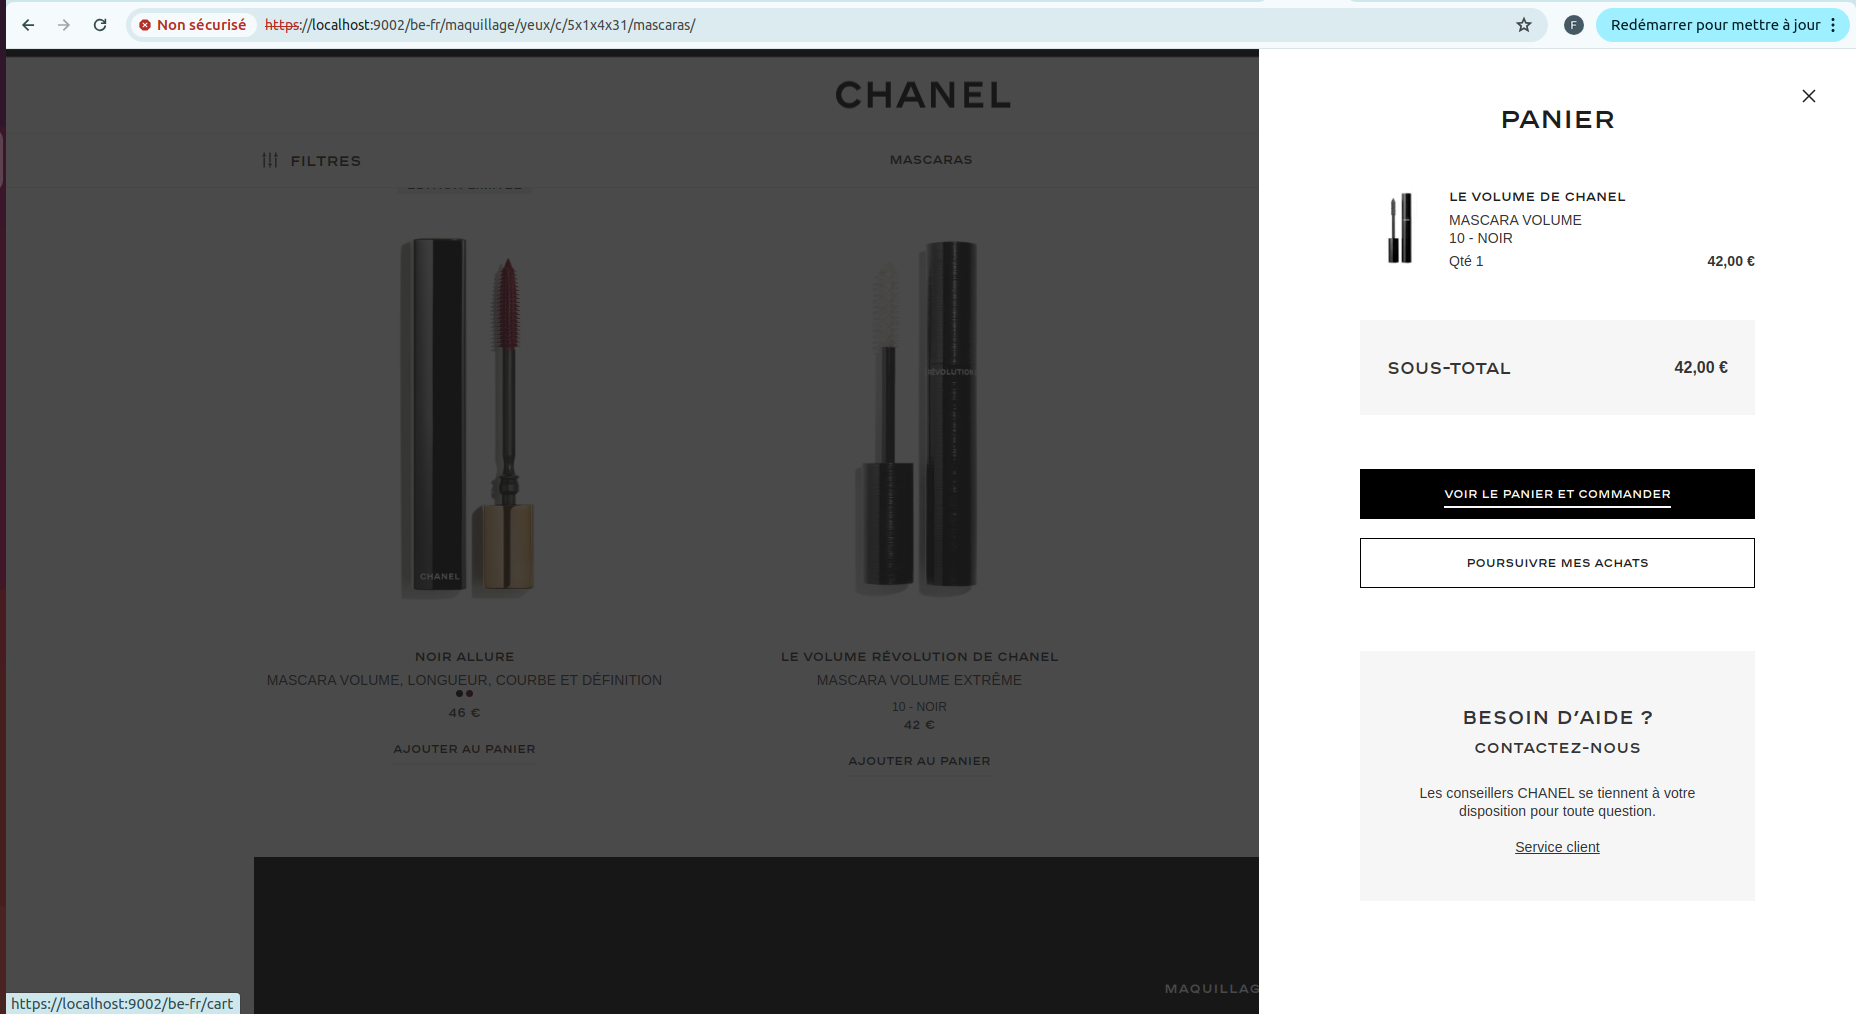
\includegraphics[width=19cm]{Figures/Screens/ajouter un produit au panier.png}
    \captionof{figure}{Ajout d'un produit au panier}
    \label{fig:selection}
\end{center}
C'est ici que commence la première étape du processus de paiement, où l'utilisateur est invité à saisir ses informations personnelles, y compris l'adresse e-mail, comme le montre la figure \ref{fig:saisie}.
\begin{center}
    \centering
    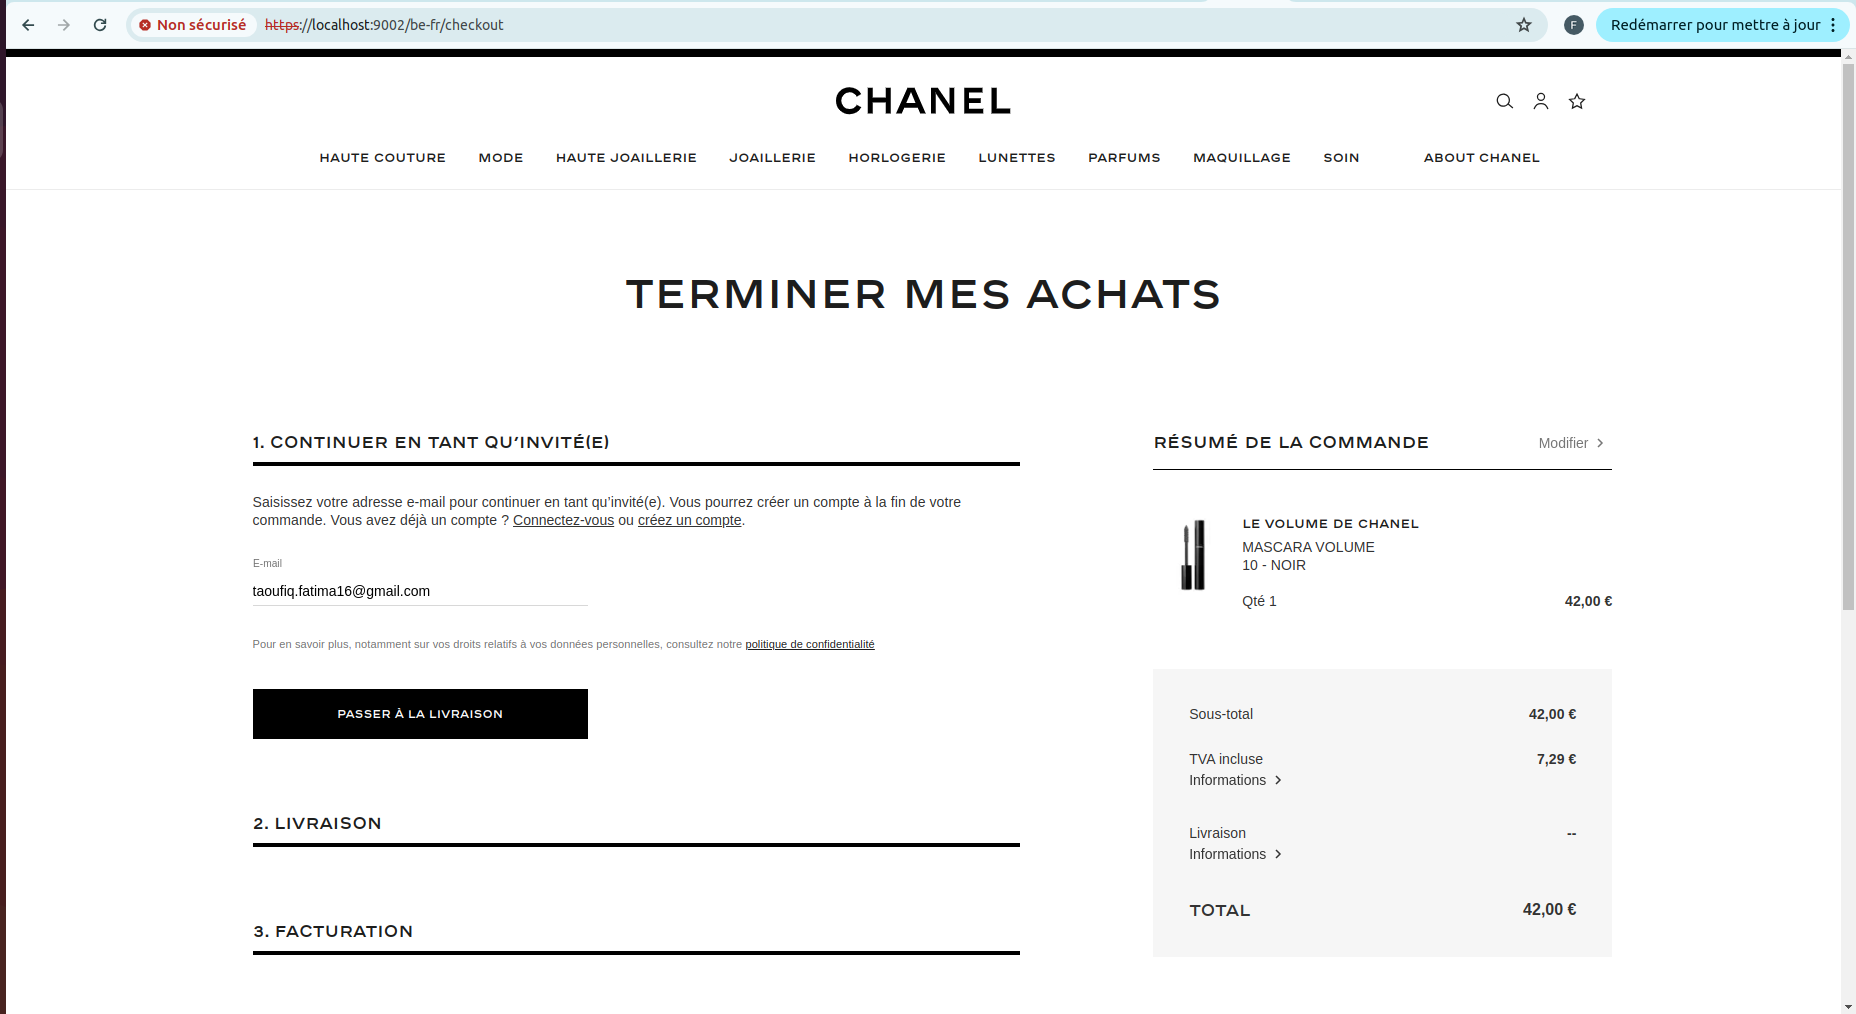
\includegraphics[width=19cm]{Figures/Screens/ajout de l'email.png}
    \captionof{figure}{Saisir les informations personnelles}
    \label{fig:saisie}
\end{center}
Après avoir rempli ses informations personnelles, l'utilisateur passe à la deuxième étape du processus de paiement, dédiée à la sélection du mode de livraison. Comme illustré dans la figure \ref{fig:mode}, cette étape permet à l'utilisateur de choisir entre la livraison à domicile ou le retrait en magasin (Click \& Collect). 
En fonction de l'option sélectionnée, l'interface offre les champs nécessaires : pour la livraison à domicile, l'utilisateur doit Saisir une adresse complète, tandis que pour le retrait en magasin, il choisit le point de retrait souhaité. Cette personnalisation assure une expérience de commande adaptée aux préférences de livraison de chaque utilisateur.
\begin{center}
    \centering
    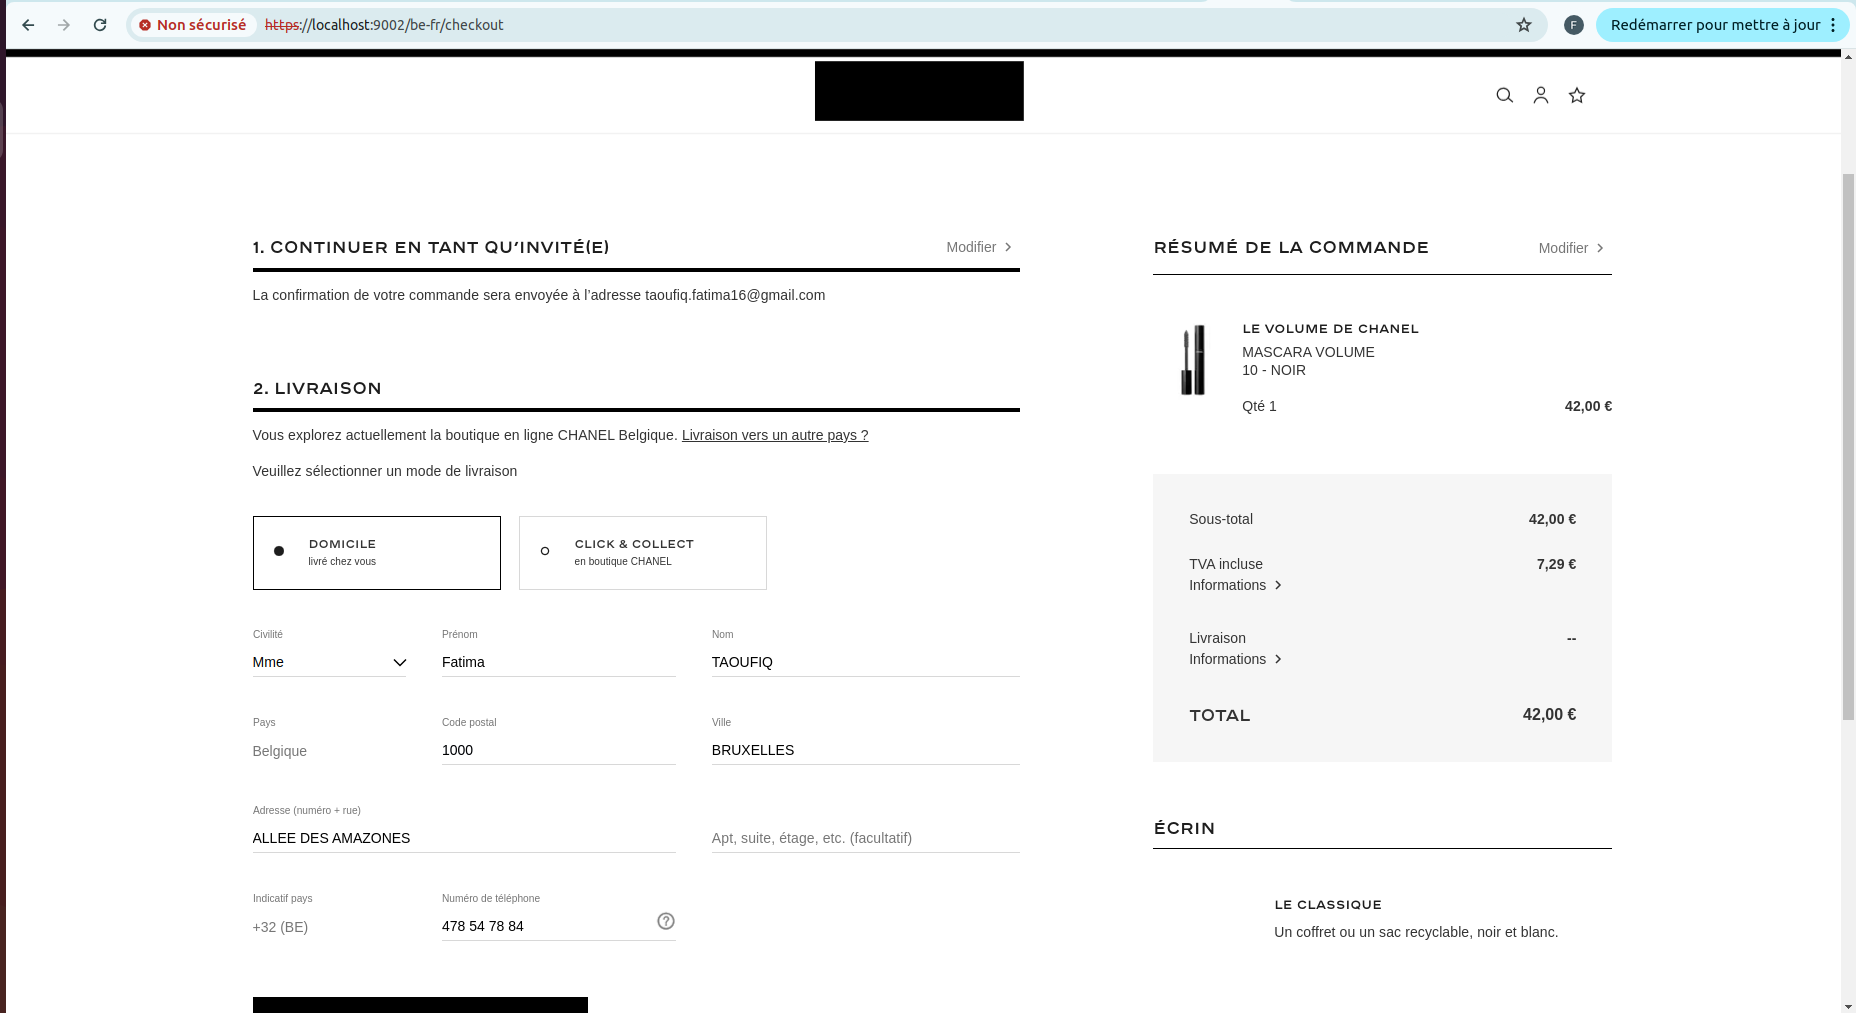
\includegraphics[width=19cm]{Figures/Screens/Infos livraison.png}
    \captionof{figure}{Mode de livraison}
    \label{fig:mode}
\end{center}
Si un code promotionnel est disponible, l'utilisateur peut l'entrer dans le champ prévu à cet effet (\textit{Figure \ref{fig:promo}}) pour bénéficier d'une réduction. 
\begin{center}
    \centering
    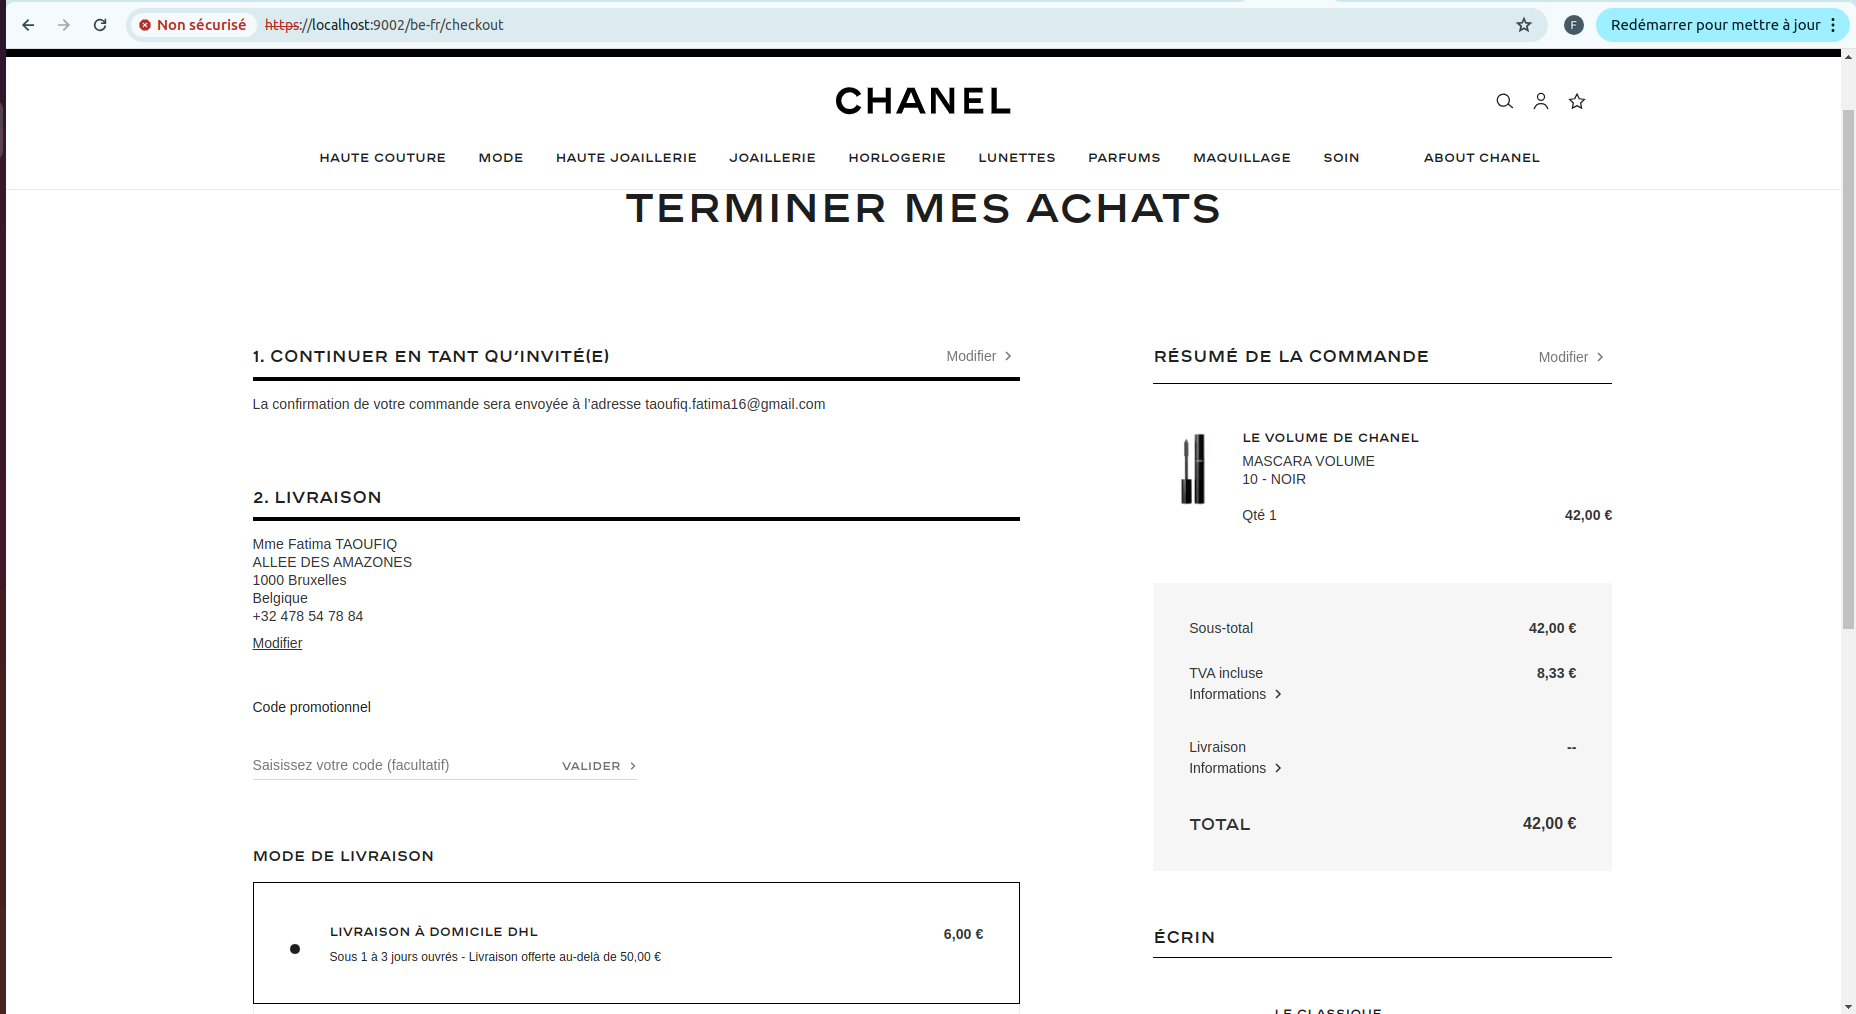
\includegraphics[width=19cm]{Figures/Screens/code prommo.png}
    \captionof{figure}{Saisir un code promo}
    \label{fig:promo}
\end{center}
En l'absence de code, l'utilisateur poursuit directement vers l'étape suivante : la facturation. À ce stade, il est invité à saisir ses informations de facturation. L'interface (\textit{Figure \ref{fig:facturation}}) propose de reprendre automatiquement l'adresse de livraison pour simplifier le processus, mais permet également de renseigner une adresse différente si nécessaire. Cette flexibilité assure que les informations de facturation peuvent être adaptées selon les besoins de l'utilisateur, tout en garantissant que les détails de facturation restent distincts de ceux de la livraison, si tel est le souhait.
\begin{center}
    \centering
    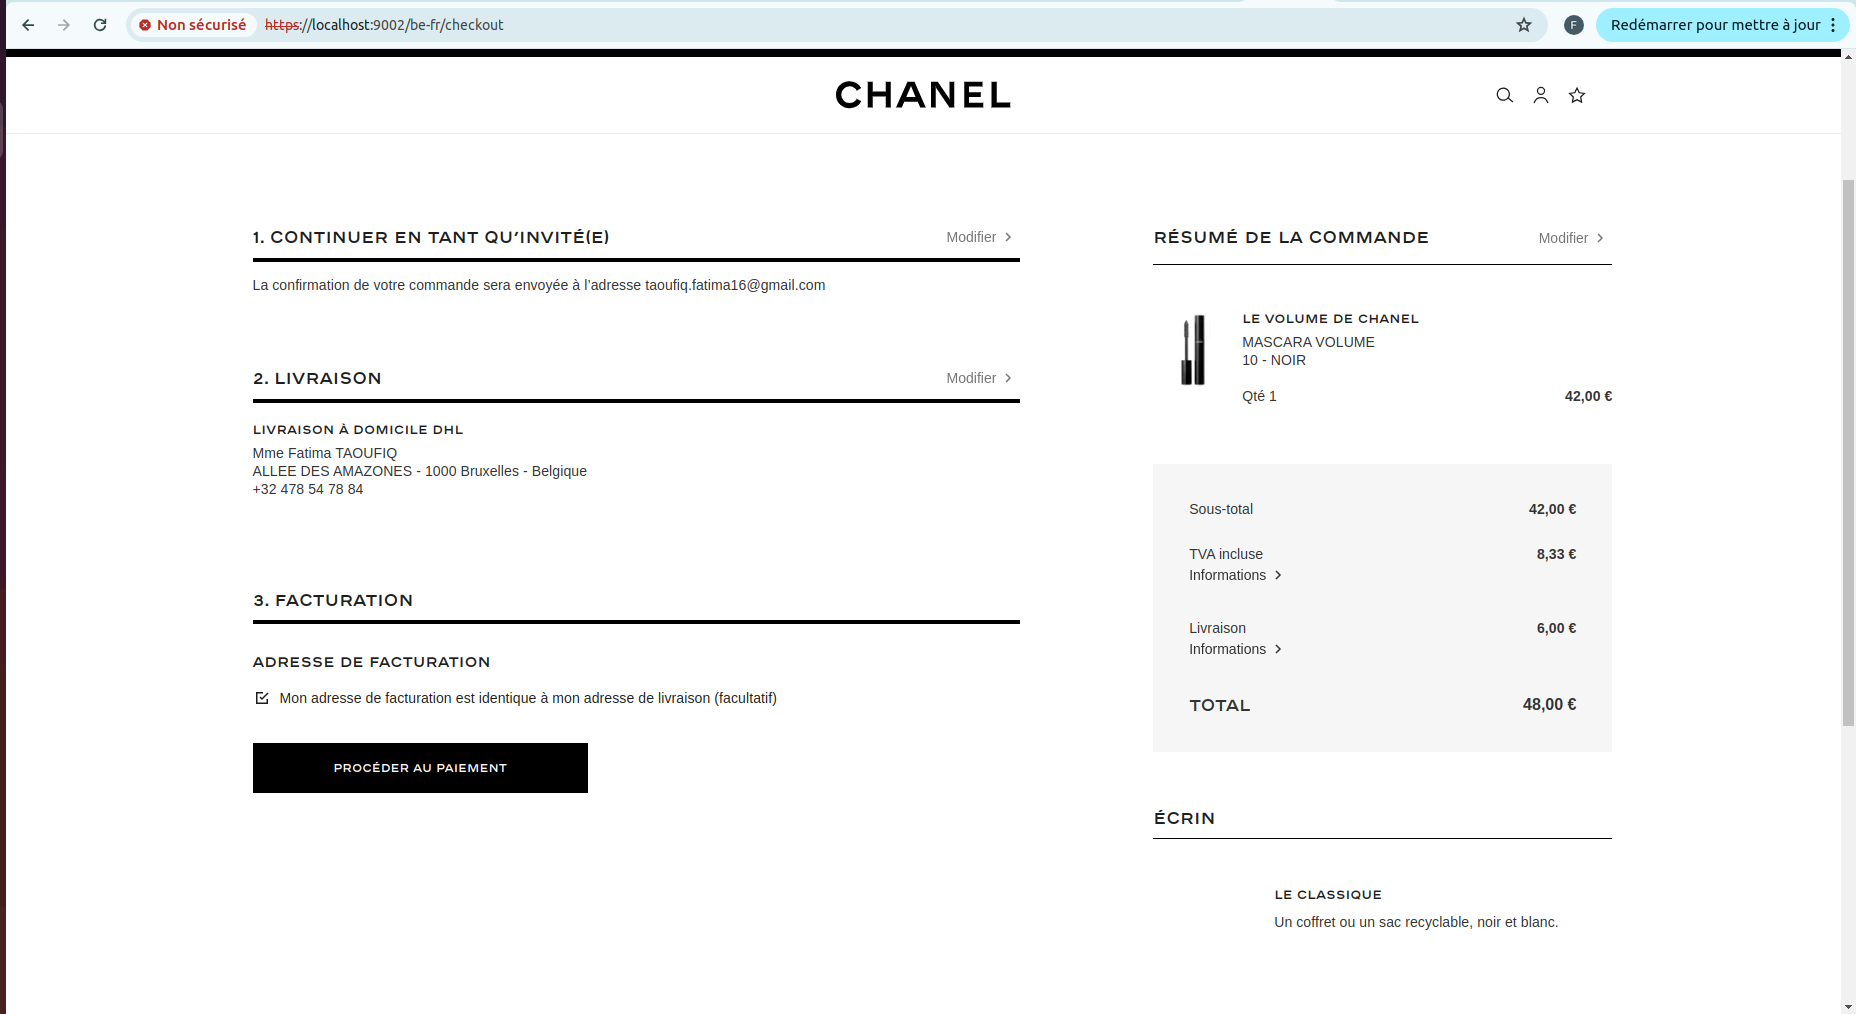
\includegraphics[width=19cm]{Figures/Screens/passe au facturation.png}
    \captionof{figure}{Facturation}
    \label{fig:facturation}
\end{center}
Après que le client a complété toutes ses informations de facturation, il accède à l'interface de sélection des modes de paiement(\textit{Figure \ref{fig:mode_paiement}}). À cette étape, il peut choisir parmi plusieurs options disponibles, y compris Payconiq, qui est mise en avant comme méthode de paiement. 
L'interface est conçue pour faciliter le choix de la méthode préférée par l'utilisateur avant de procéder à l'étape suivante du processus de paiement.
\begin{center}
    \centering
    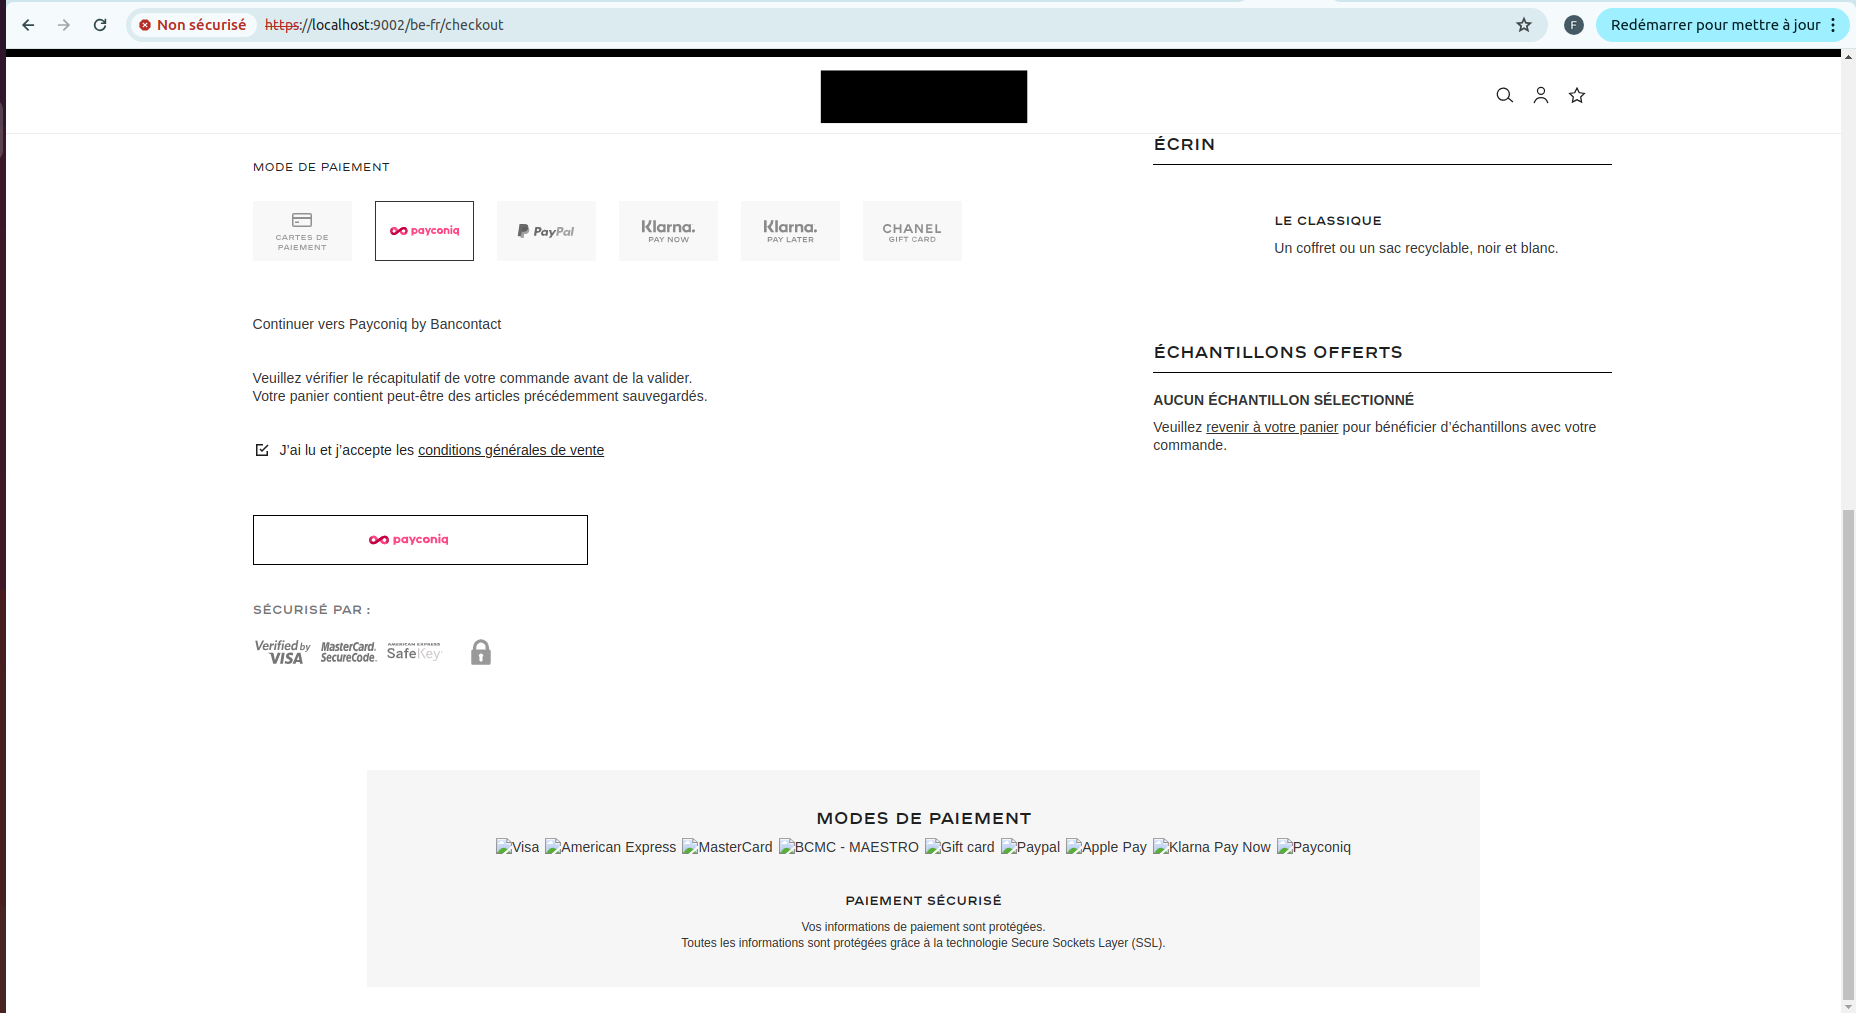
\includegraphics[width=19cm]{Figures/Screens/payment.png}
    \captionof{figure}{Choix de mode de paiement}
    \label{fig:mode_paiement}
\end{center}
Après avoir sélectionné le mode de paiement, l'utilisateur est dirigé vers l'API Adyen. Sur cette interface, un QR code est généré pour finaliser la transaction. Comme l'illustre la figure \ref{fig:qr}, ce QR code doit être scanné dans les 15 minutes pour éviter l'annulation automatique de la commande. L'interface fournit également un compte à rebours indiquant le temps restant pour effectuer le paiement, garantissant ainsi une expérience utilisateur fluide et sécurisée.
\begin{center}
    \centering
    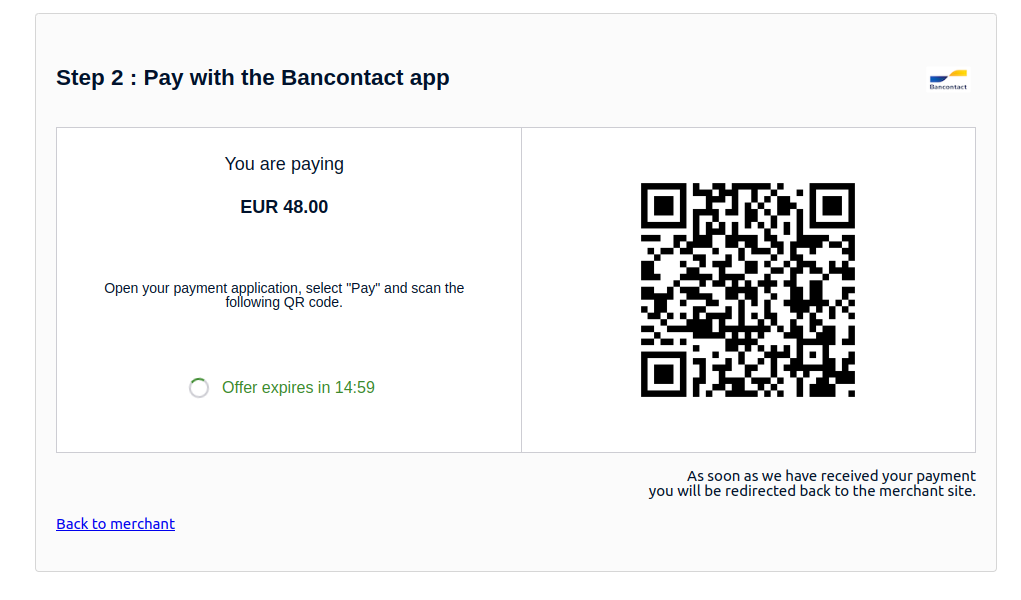
\includegraphics[width=19cm]{Figures/Screens/redirection.png}
    \captionof{figure}{Finalisation du paiement via l'API Adyen}
    \label{fig:qr}
\end{center}
Une fois redirigé vers la page de paiement, l'utilisateur traverse plusieurs étapes :
Tout d'abord, il est accueilli par un écran indiquant qu'il doit patienter pendant que la transaction est traitée. 
\begin{center}
    \centering
    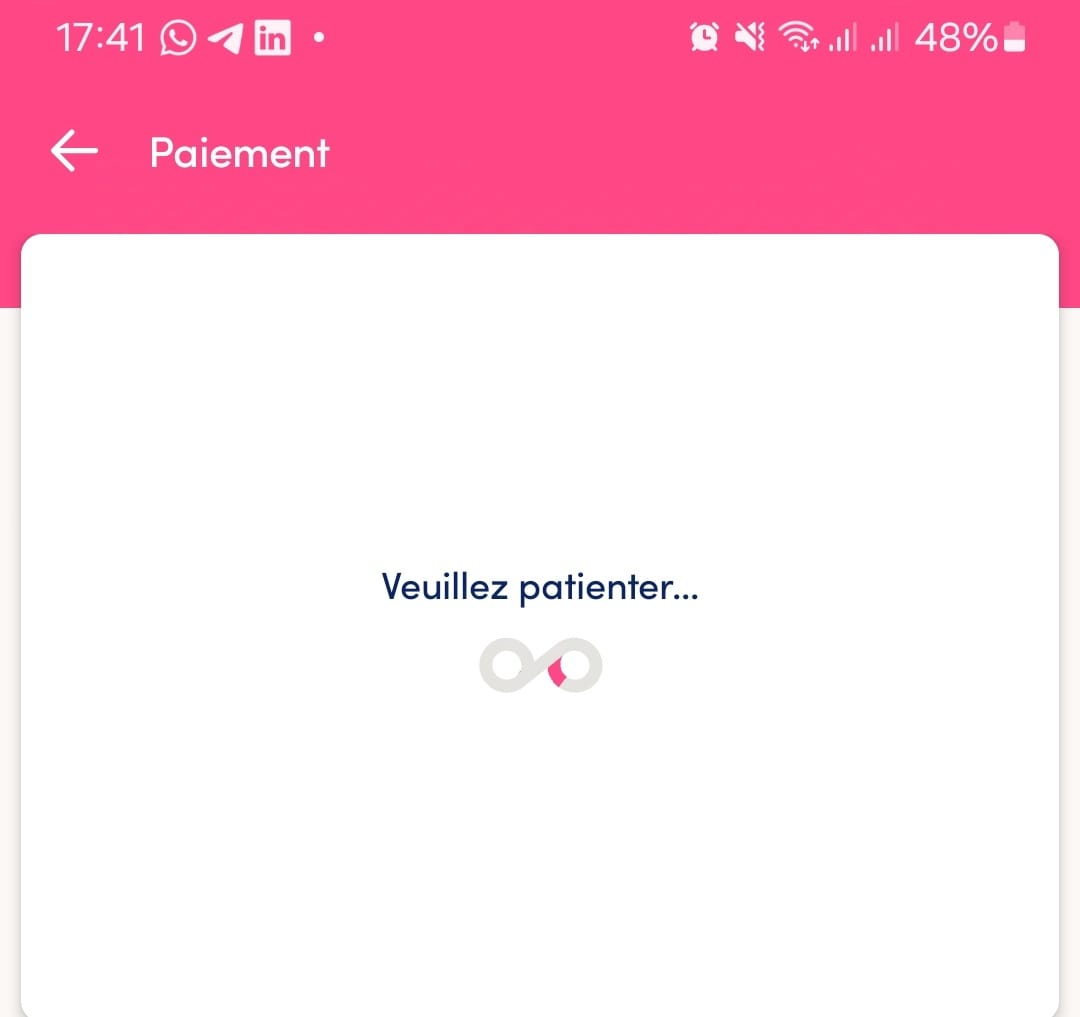
\includegraphics[width=10cm]{Figures/Screens/patience.jpeg}
    \captionof{figure}{Écran de traitement en cours}
    \label{fig:patience}
\end{center}
Ensuite, l'écran suivant affiche le montant total à payer et demande a l'utilisateur d'autoriser la transaction, comme le montre la figure \ref{fig:autorisation}
\begin{center}
    \centering
    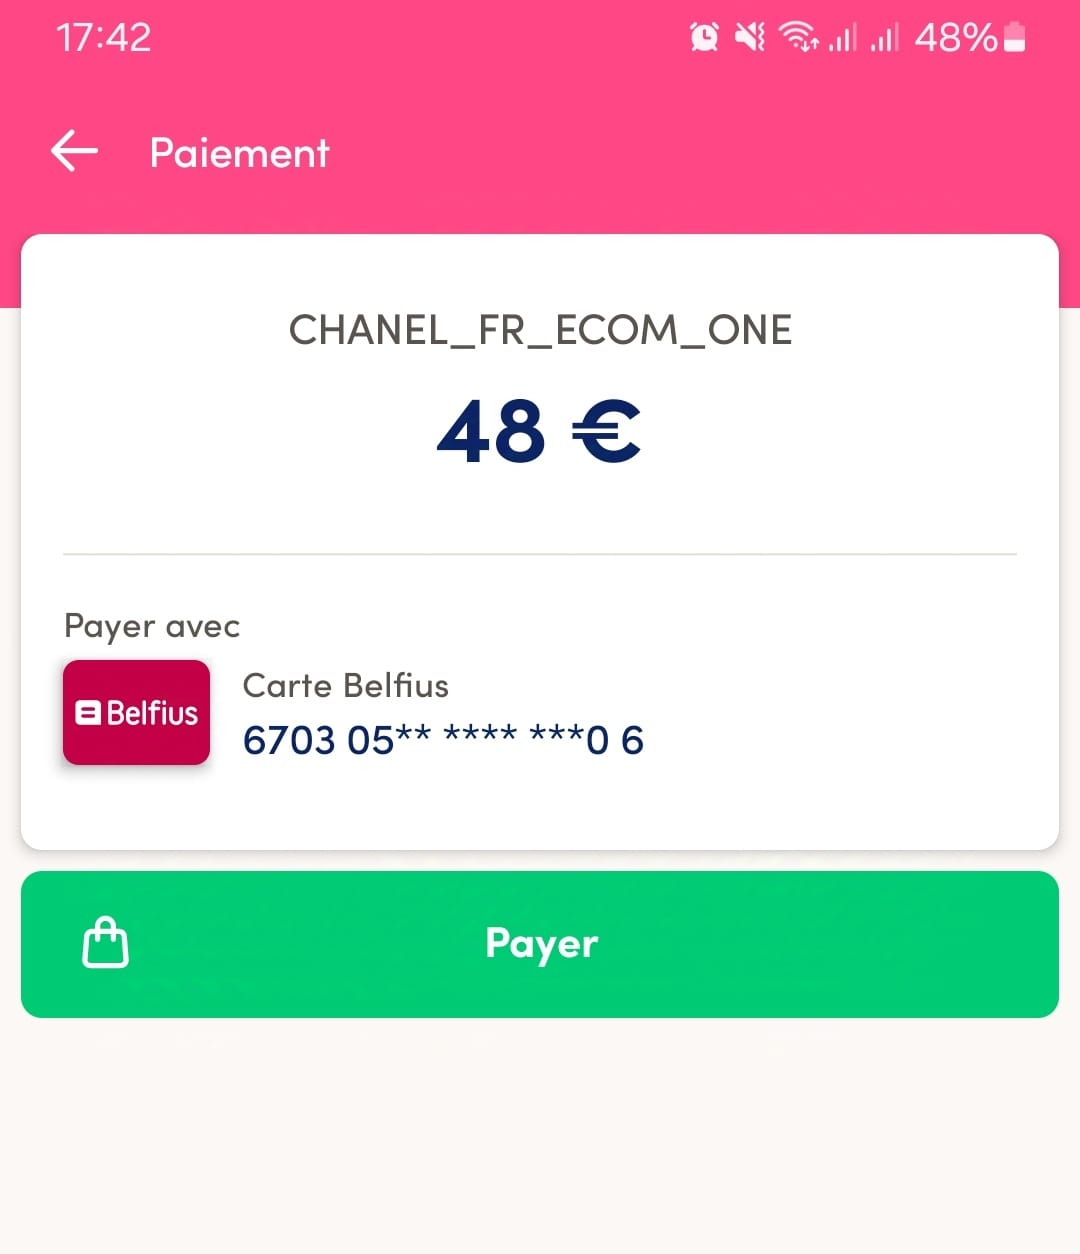
\includegraphics[width=10cm]{Figures/Screens/montant.jpeg}
    \captionof{figure}{Montant à payer}
    \label{fig:autorisation}
\end{center}
Enfin, lorsque la transaction est réussie, l'utilisateur est redirigé vers un écran de confirmation de paiement, illustré dans la figure \ref{fig:reussie}
\begin{center}
    \centering
    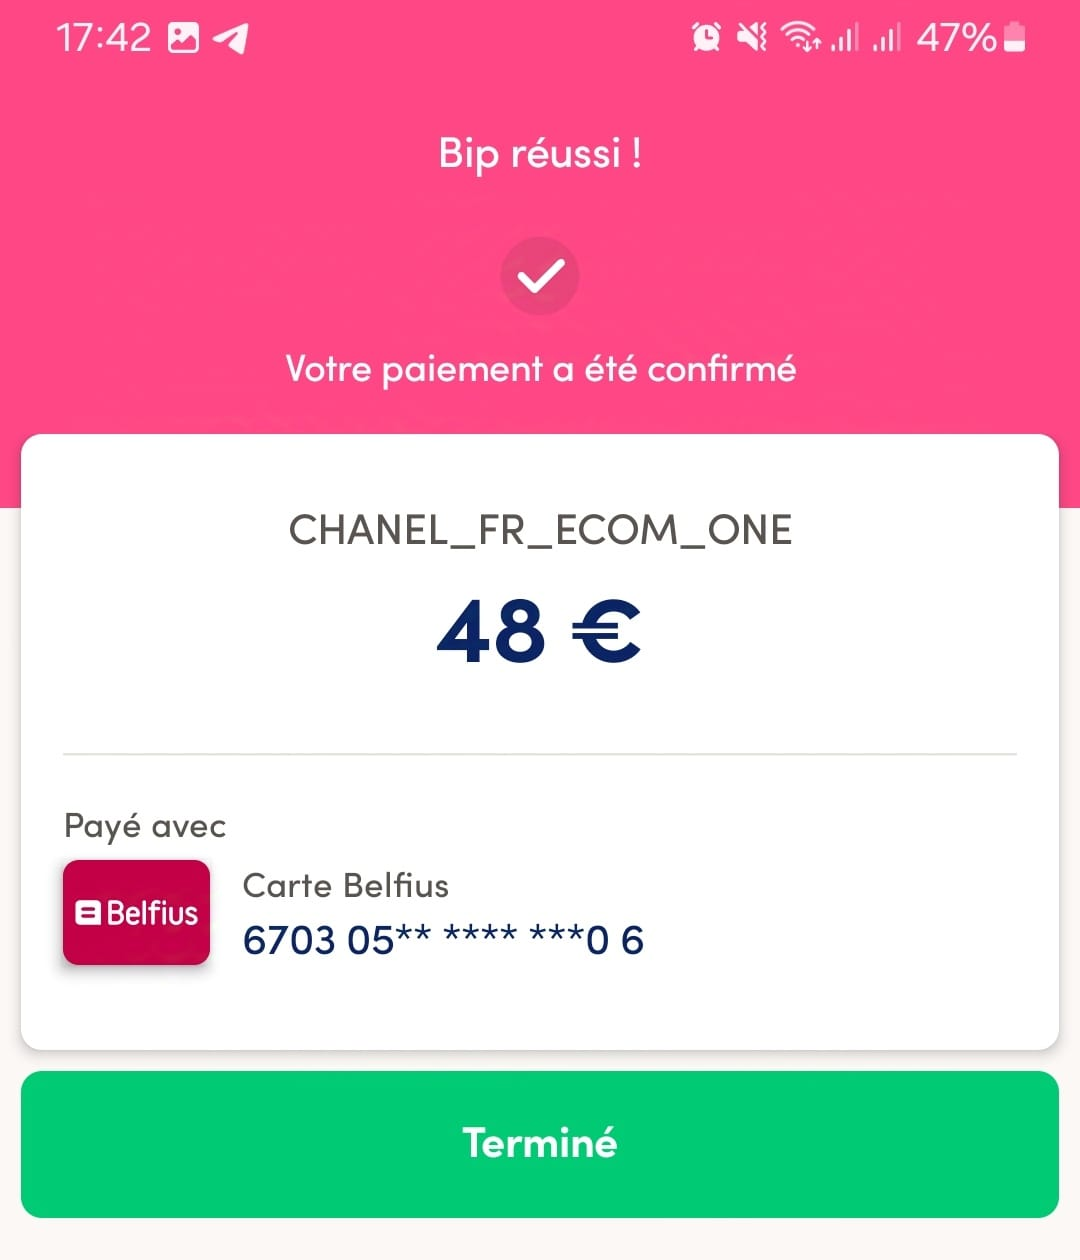
\includegraphics[width=10cm]{Figures/Screens/reussi.jpeg}
    \captionof{figure}{Paiement reussi}
    \label{fig:reussie}
\end{center}
Après la finalisation réussie du paiement, l'utilisateur est dirigé vers une page de confirmation de commande (\textit{Figure \ref{fig:confirmation}}). Cette page présente un identifiant unique de suivi, facilitant le suivi de l'état de la commande. 
\begin{center}
    \centering
    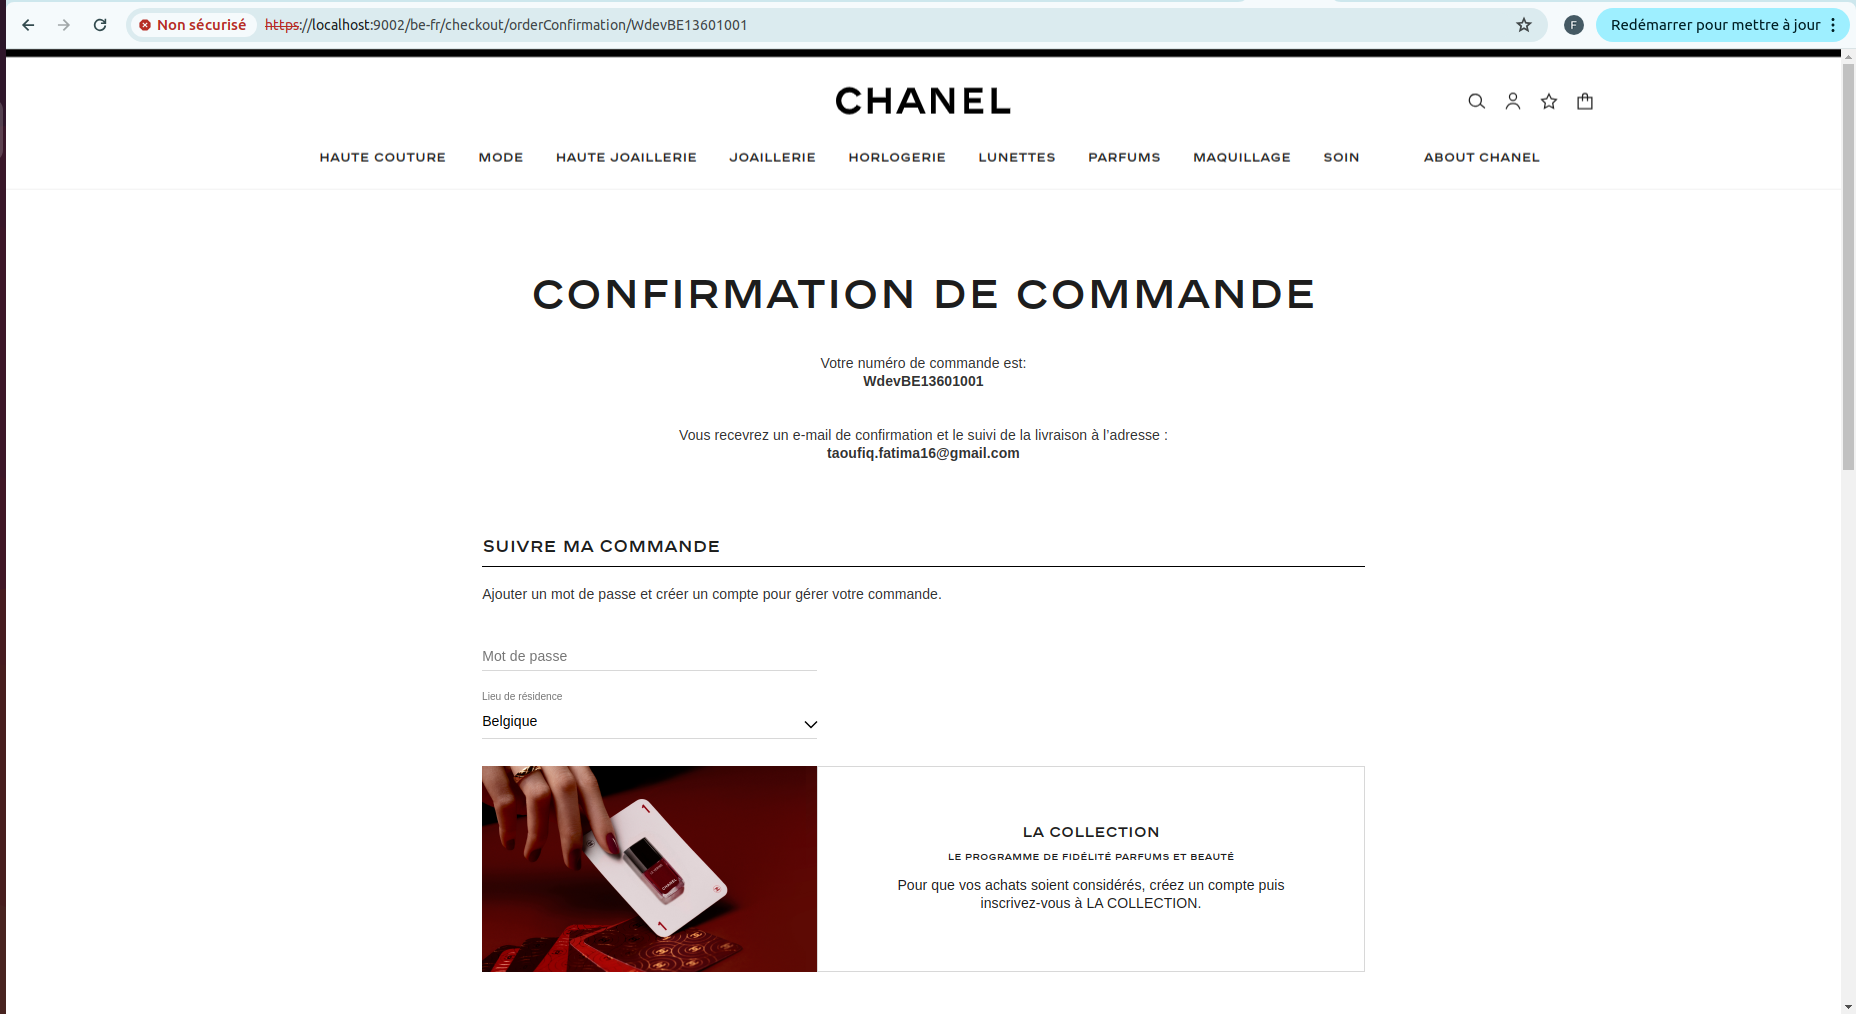
\includegraphics[width=19cm]{Figures/Screens/confirmation du commande.png}
    \captionof{figure}{Confirmation de la commande}
    \label{fig:confirmation}
\end{center}
En plus de cet identifiant, toutes les informations nécessaires sont fournies (\textit{Figure \ref{fig:resume}}), telles que l'email pour le suivi de la livraison. L'interface propose également des options pour gérer la commande, notamment la possibilité de créer un compte utilisateur pour un accès facilité aux informations de commande et aux fonctionnalités associées.
\begin{center}
    \centering
    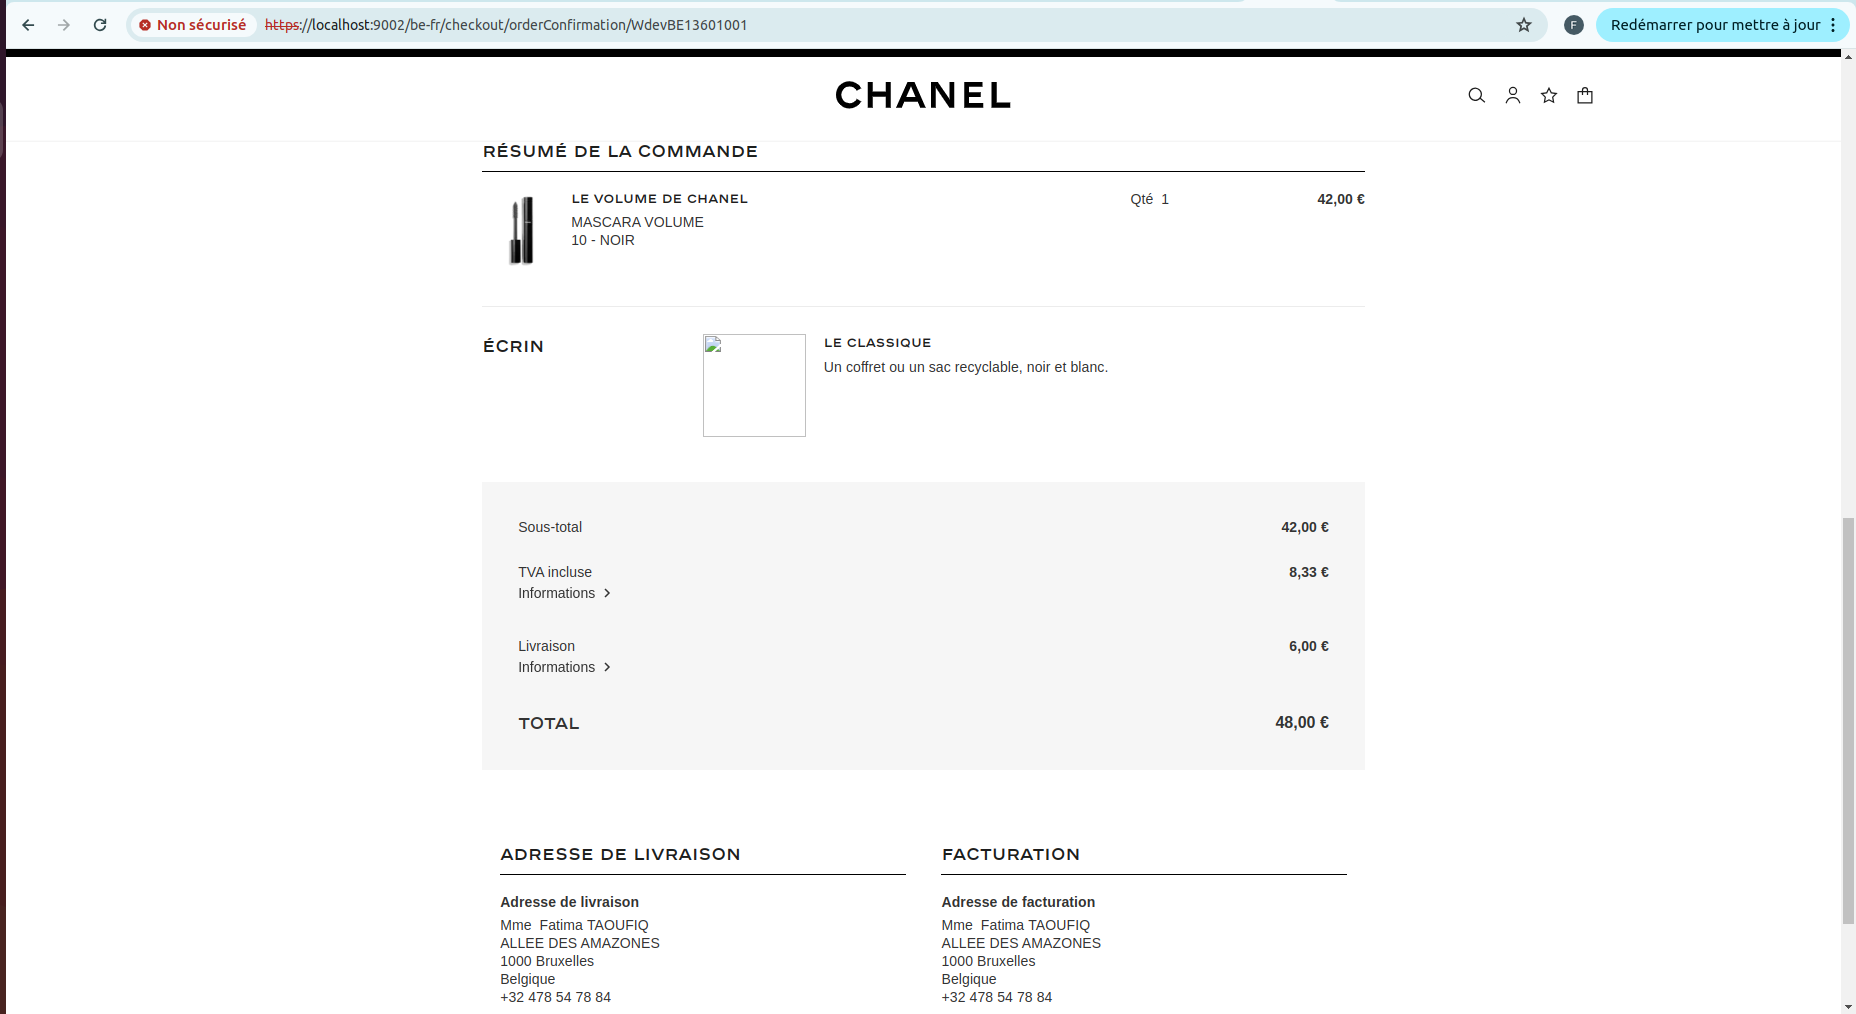
\includegraphics[width=19cm]{Figures/Screens/resumer commande.png}
    \captionof{figure}{Informations de la commande}
    \label{fig:resume}
\end{center}
En cas d'annulation ou de non-approbation du paiement, la page de confirmation de commande affichera un message d'erreur détaillé. Comme le montre la figure \ref{fig:erreur}, un avertissement est clairement indiqué : "Remarque : les informations de paiement sont erronées. Veuillez vérifier ces informations afin de confirmer votre commande." Ce message signifie que le processus de validation du paiement n'a pas été complété correctement, nécessitant une révision des informations saisies pour procéder à la confirmation de la commande.
\begin{center}
    \centering
    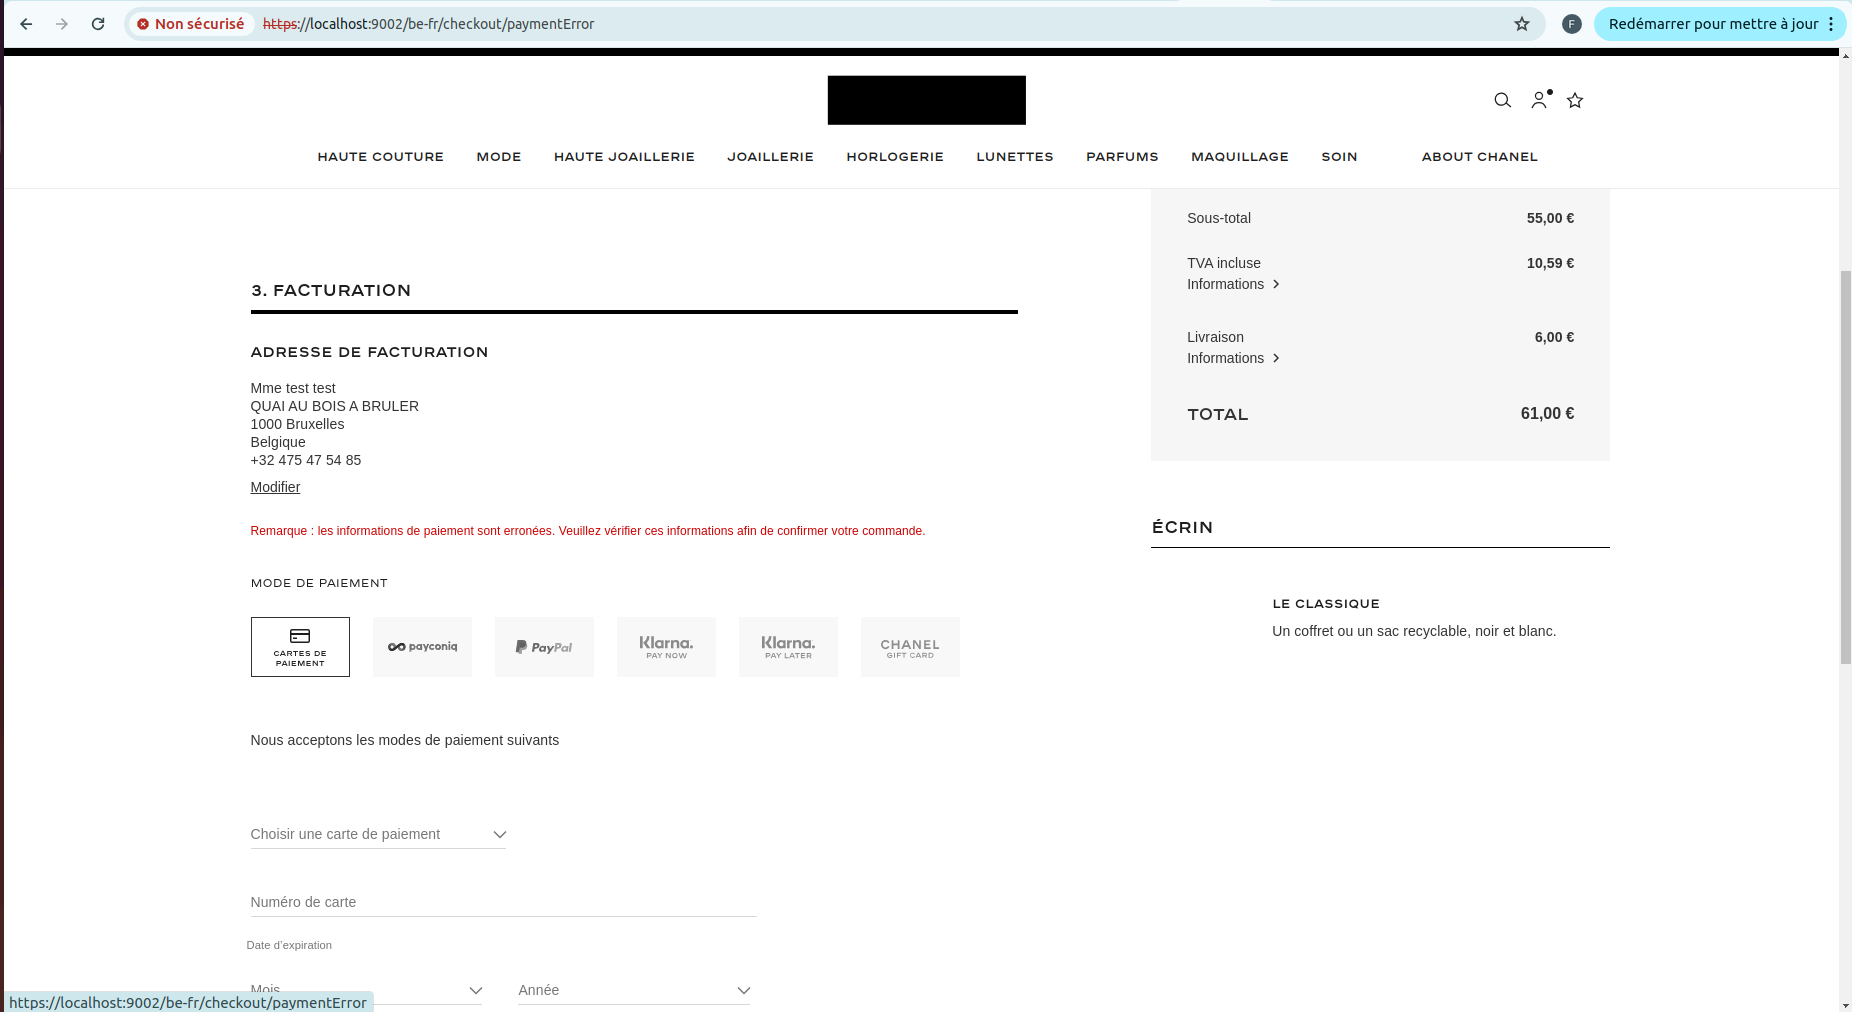
\includegraphics[width=19cm]{Figures/Screens/annulation de commande.png}
    \captionof{figure}{Message d'erreur en cas d'annulation du paiement}
    \label{fig:erreur}
\end{center}
Si la commande est effectuée avec succès, la figure \ref{fig:admin} illustre l'interface backoffice qui confirme la création de la commande et la validation réussie du paiement. Dans cet écran, l'administrateur peut consulter les détails de la commande, s'assurer que le paiement a été correctement traité et apporter toute modification nécessaire. Cette étape est essentielle pour le suivi du processus de commande et permet de gérer efficacement les commandes après l'autorisation du paiement.
\begin{center}
    \centering
    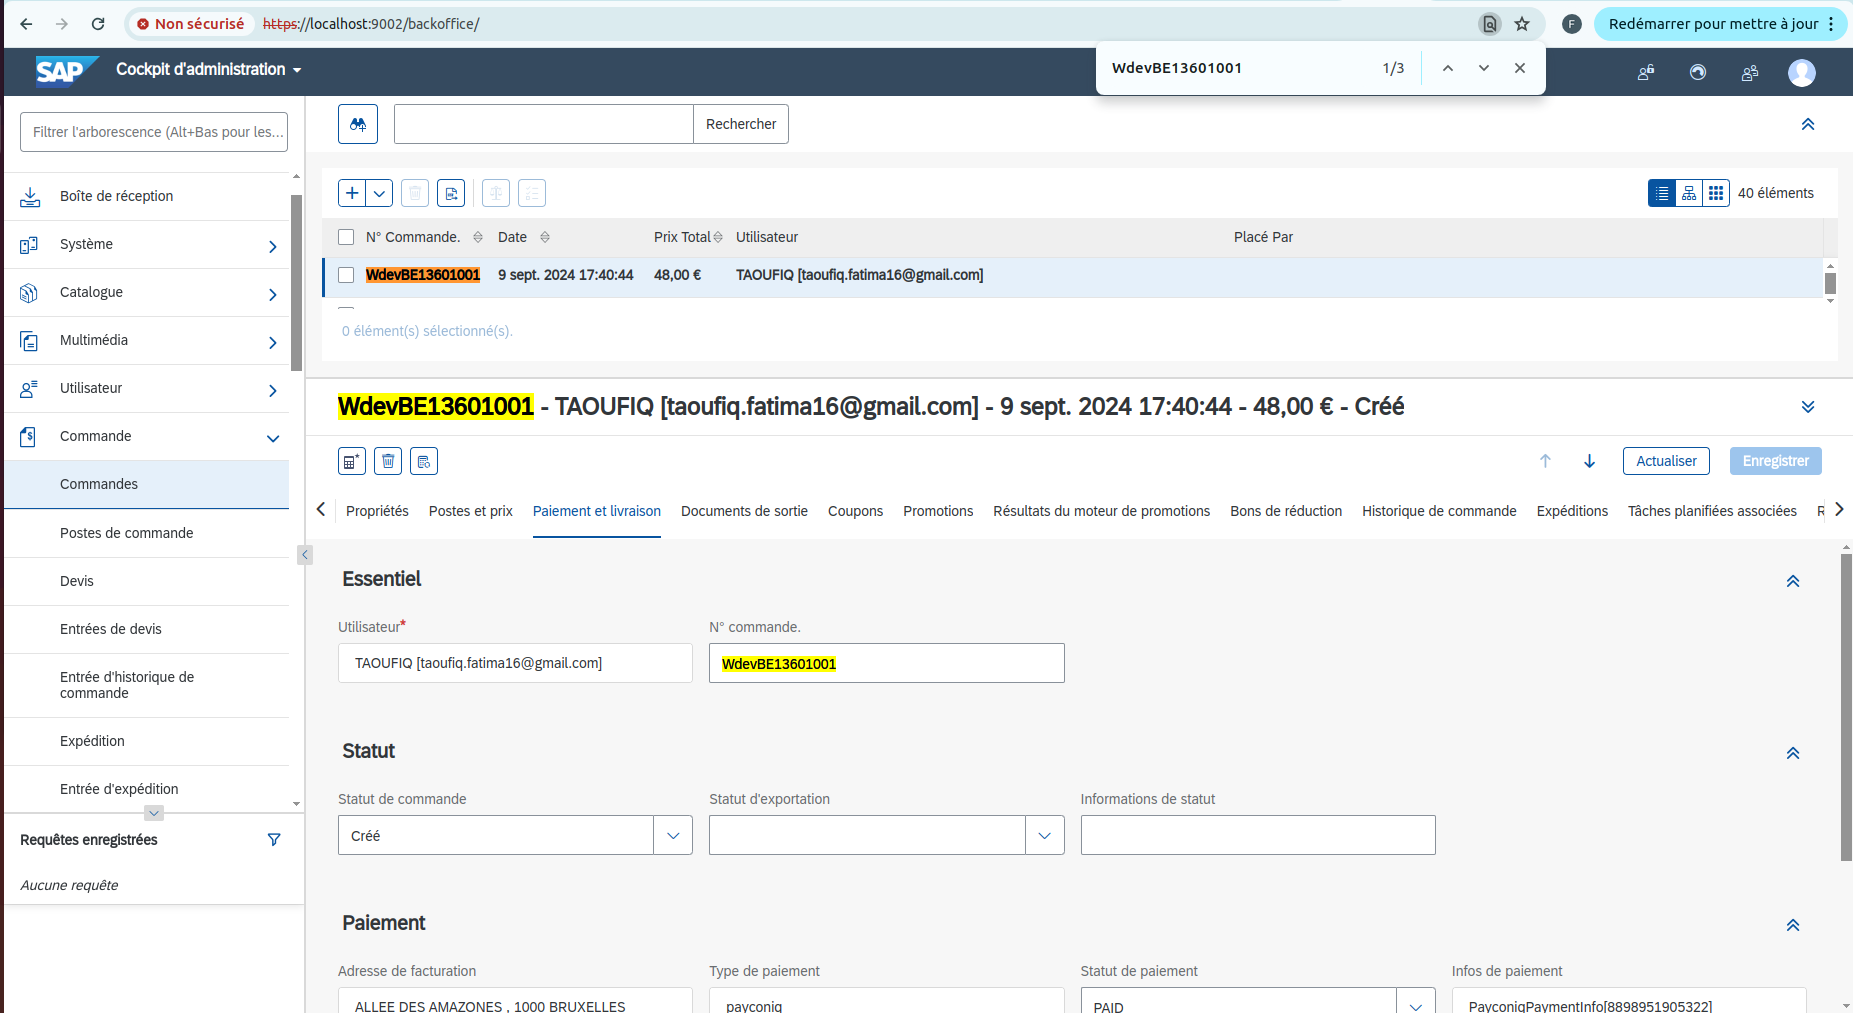
\includegraphics[width=19cm]{Figures/Screens/Backoffice commande.png}
    \captionof{figure}{Confirmation de la commande dans le backoffice}
    \label{fig:admin}
\end{center}
Une fois la commande validée, un e-mail est automatiquement envoyé à l'utilisateur, confirmant les détails de l'achat et assurant une traçabilité complète. Ce message inclut des informations essentielles telles que le numéro de commande, les articles achetés, le montant total, ainsi que les coordonnées de livraison. Cette étape permet à l'utilisateur de suivre sa commande de manière transparente et de vérifier les détails importants relatifs à son achat.
\begin{center}
    \centering
    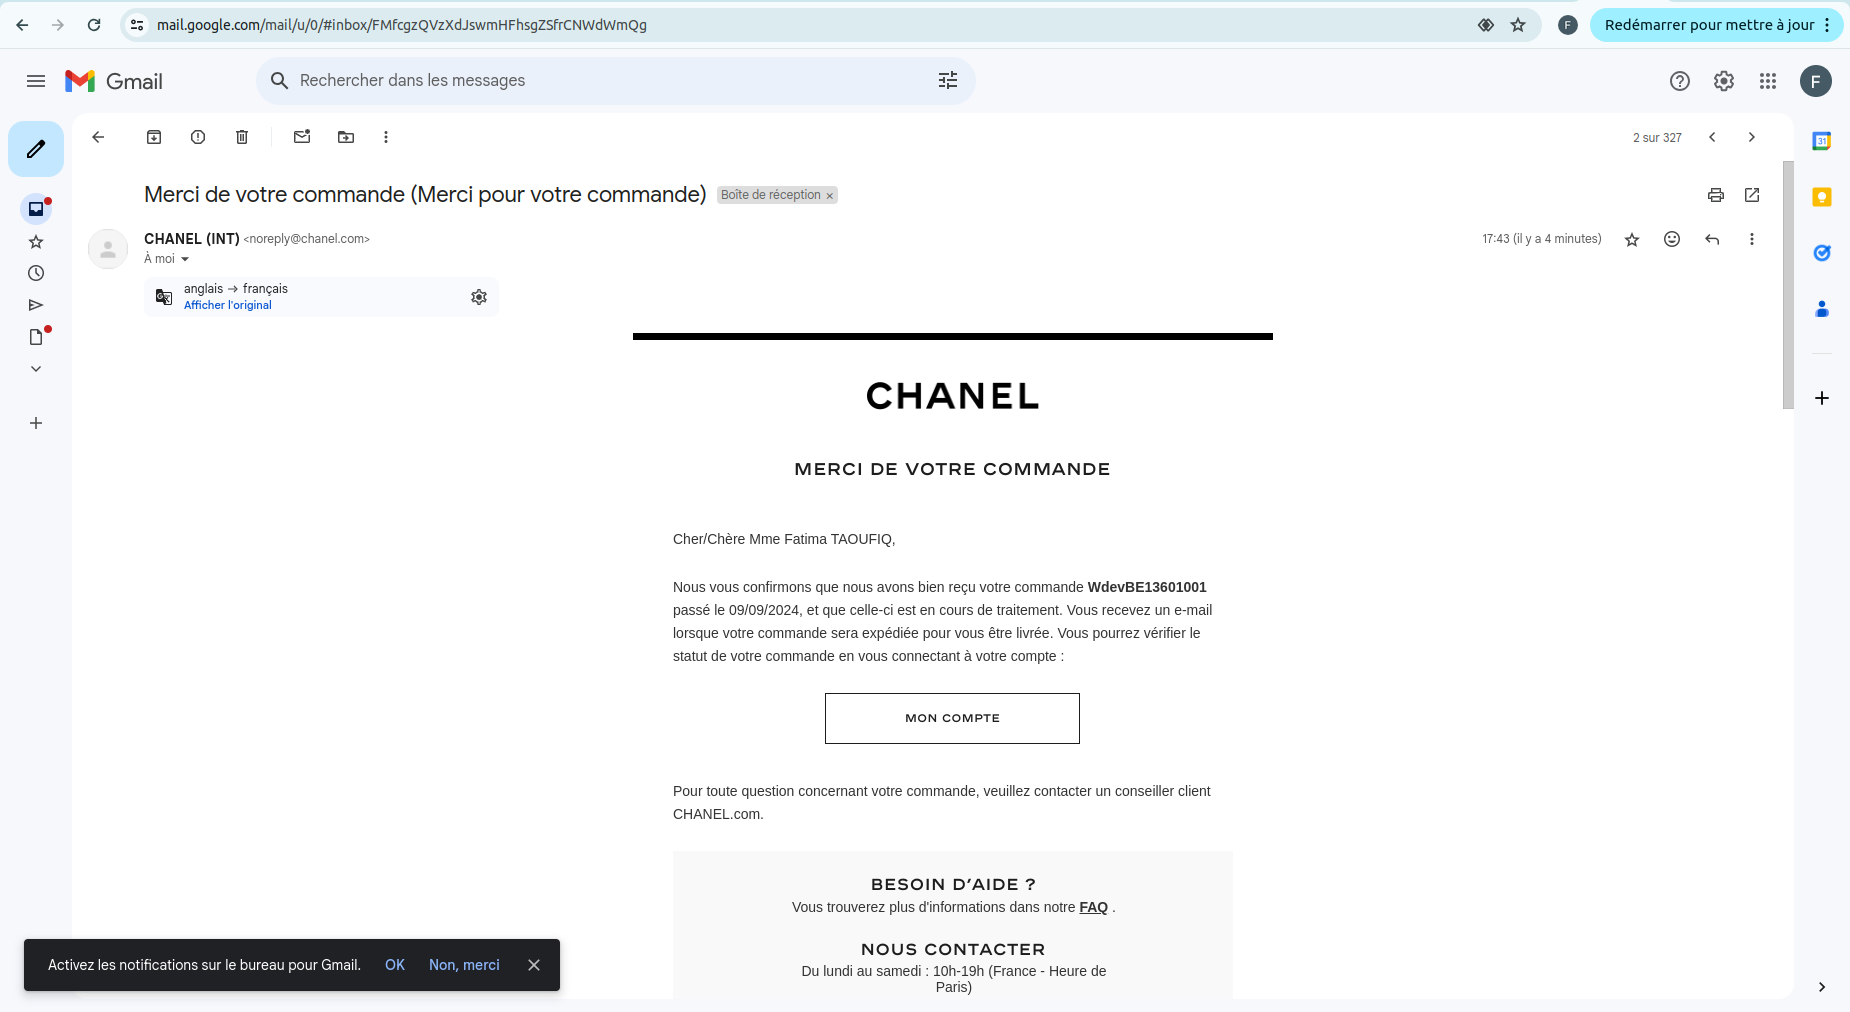
\includegraphics[width=19cm]{Figures/Screens/confirmation par mail.png}
    \captionof{figure}{Message de confirmation par email}
    \label{fig:email}
\end{center}
\section{Analyse et Correction des Anomalies}

Au cours de cette période, une partie essentielle de mon travail a consisté à résoudre les problèmes détectés par SonarQube, un outil d'analyse statique qui permet d'améliorer la qualité du code. Comme illustré par les captures ci-dessous, SonarQube a mis en évidence plusieurs anomalies critiques, notamment des  duplications de littéraux  et des  complexités cognitives  élevées dans certaines méthodes du projet. Ces problèmes, jugés critiques, nécessitaient une attention immédiate pour garantir une bonne maintenabilité du projet.

En corrigeant ces anomalies, j'ai non seulement amélioré la maintenabilité du projet, mais aussi réduit les risques d'erreurs futures. Ce travail d'optimisation a permis de renforcer la  robustesse  du code et d'assurer que le projet respecte les bonnes pratiques de développement logiciel, en ligne avec les normes de qualité du secteur.
\begin{center}
    \centering
    \includegraphics[width=19cm]{Figures/Screens/bug.png}
    \captionof{figure}{Bugs détectés par SonarQube}
    \label{fig:corr}
\end{center}
Pour corriger ces bugs critiques, plusieurs bonnes pratiques ont été mises en œuvre, notamment :

\begin{itemize}
    \item[$\bullet$] \textbf{Extraction des chaînes de caractères répétitives} : Les chaînes de caractères fréquemment répétées dans le code ont été isolées et déclarées sous forme de variables constantes, réduisant ainsi la redondance et facilitant la maintenance.
    \item[$\bullet$] \textbf{Réduction de la complexité des méthodes} : Les méthodes présentant une complexité cognitive élevée ont été découpées en sous-méthodes plus simples et cohérentes, améliorant ainsi la lisibilité du code et facilitant sa compréhension.
    \item[$\bullet$] \textbf{Refactorisation du code en suivant le principe DRY (Don't Repeat Yourself)} : Les portions de code dupliquées ont été consolidées et regroupées dans des fonctions réutilisables, ce qui a permis de limiter les répétitions et d'optimiser la structure globale du projet.
\end{itemize}

Suite à une analyse avec SonarLint, nous avons vérifié que toutes les anomalies critiques ont bien été corrigées.

\begin{center}
    \centering
    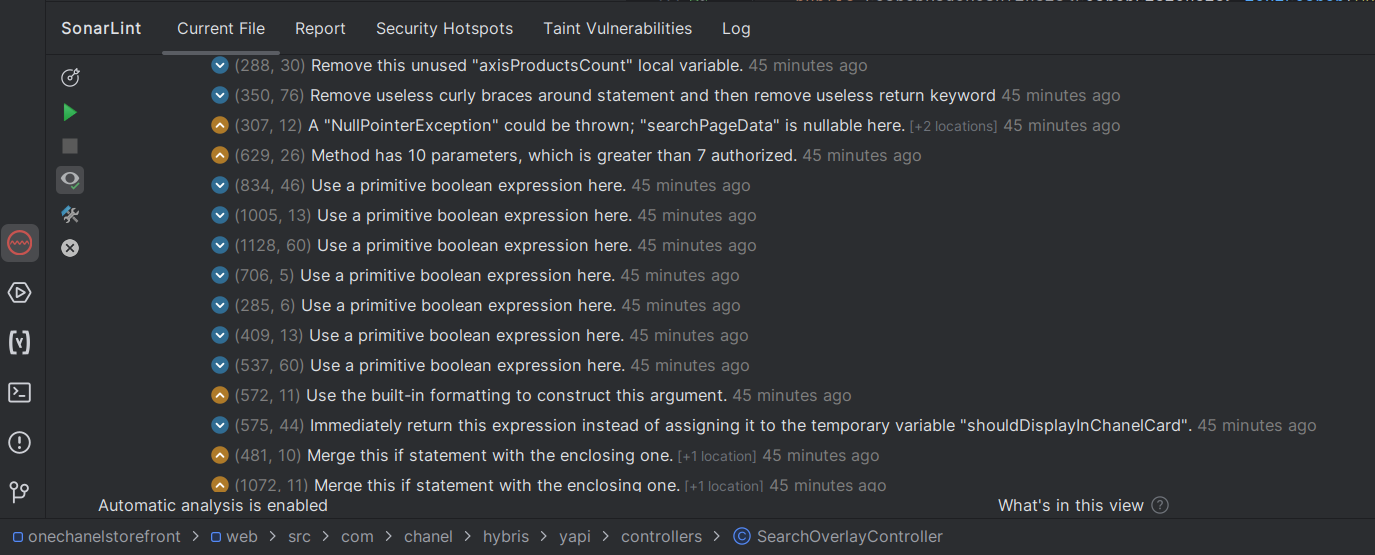
\includegraphics[width=19cm]{Figures/bug1.png}
    \captionof{figure}{Analyse avec SonarLint après correction}
\end{center}


Dans le cadre de notre analyse, nous identifions si le problème provient de notre côté, au niveau du backend, ou s'il est lié à une autre équipe. Si le problème est de notre responsabilité, nous procédons à la correction. Dans le cas où il est lié à une autre équipe, nous demandons l'association du ticket à cette dernière et veillons à leur transmettre toutes les informations nécessaires pour faciliter leur analyse.

 La figure  \ref{fig:ticket}  montre un exemple de ticket de bug utilisé pour suivre les anomalies détectées. La gestion des bugs est cruciale pour identifier et résoudre les problèmes techniques, garantissant ainsi la stabilité et la qualité du produit. Ce processus favorise également la collaboration entre les équipes, contribuant à améliorer l'expérience utilisateur.
\begin{center}
    \centering
    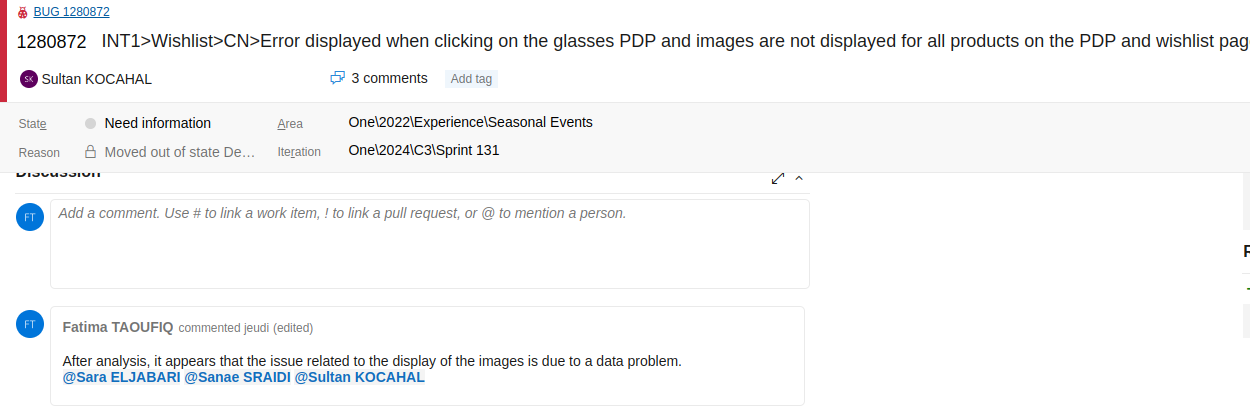
\includegraphics[width=19cm]{Figures/Screens/ticket.png}
    \captionof{figure}{Exemple ticket de debugging}
    \label{fig:ticket}
\end{center}




\section{Tests et Validation}
\subsection{Tests}
Les tests constituent une étape essentielle pour s'assurer du bon fonctionnement du système et de sa conformité aux attentes. Ils aident à repérer et corriger d'éventuelles anomalies avant la mise en production. Nous avons ainsi mené différents types de tests, allant des tests unitaires aux tests fonctionnels, réalisés sur plusieurs environnements :
\begin{itemize}
    \item[$\bullet$] \textbf{Tests unitaires :} Nous avons utilisé JUnit pour mener les tests unitaires, visant à valider chaque composant du système de manière isolée. Ces tests, réalisés en local, permettent de vérifier que les méthodes fonctionnent comme prévu, de gérer les exceptions, et d’assurer la robustesse du code avant toute intégration. Grâce à une approche rigoureuse, nous avons atteint une couverture de 100\% du code, comme le montrent les captures d'écran ci-dessous. Cette couverture complète assure que chaque ligne de code a été testée et contribue à la fiabilité globale du système.
    \begin{center}
        \centering
        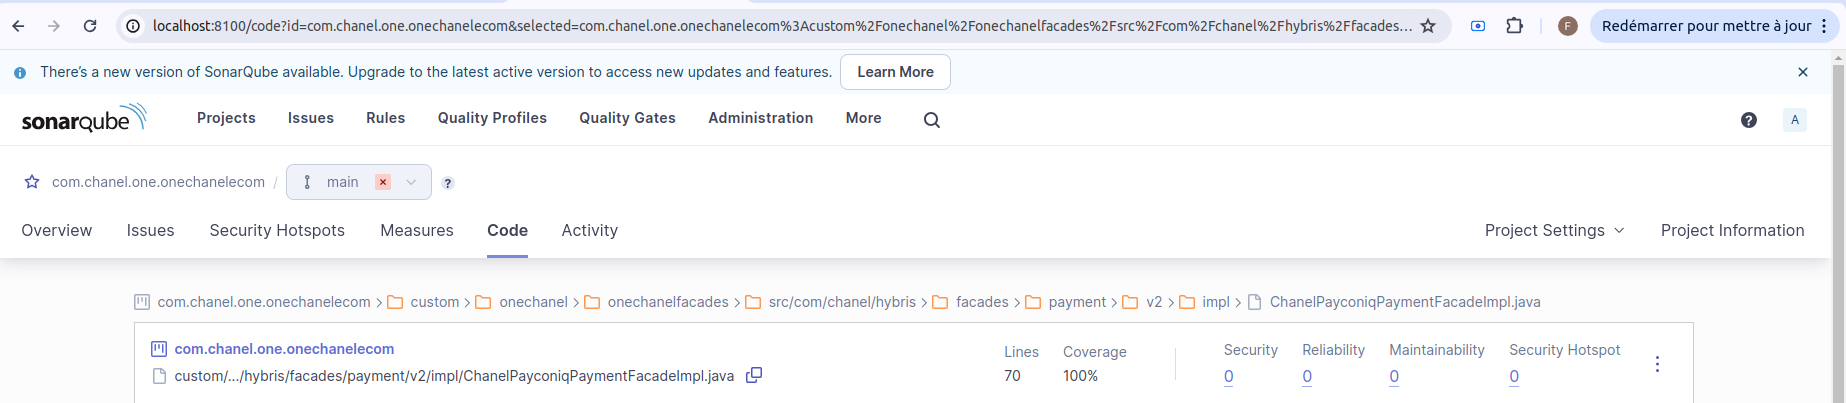
\includegraphics[width=18cm]{Figures/Screens/couvrage.png}
        \captionof{figure}{Couverture de code à 100\%}
        \label{fig:couvrage}
    \end{center}
    \begin{center}
        \centering
        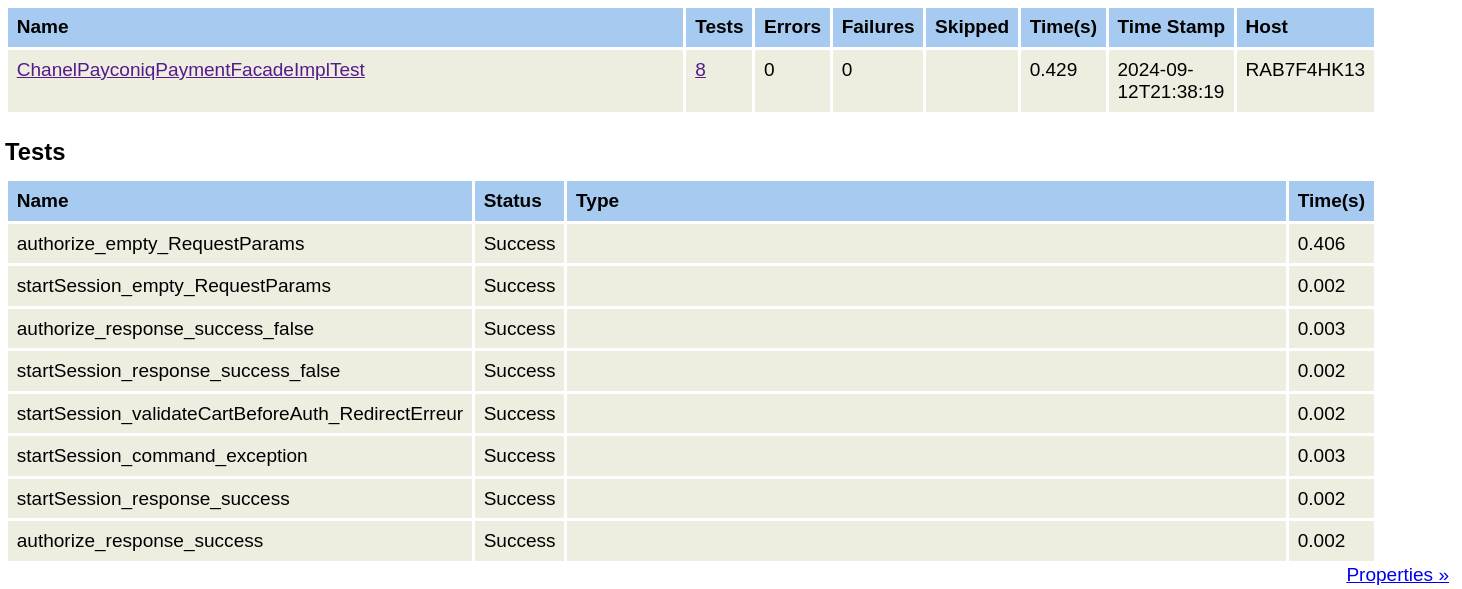
\includegraphics[width=18cm]{Figures/Screens/reportSonar.png}
        \captionof{figure}{Succès de tous les cas de test}
        \label{fig:report}
    \end{center}
    \item[$\bullet$] \textbf{Tests fonctionnels :} Les tests fonctionnels ont été pris en charge par l'équipe QA sur plusieurs environnements, tels que INT2, INT1, UAT et OAT. Ces tests permettent de valider que les fonctionnalités développées respectent les exigences métiers et opèrent correctement dans des conditions réalistes. INT1 est utilisé comme environnement partagé par toutes les équipes, tandis que INT2 est dédié à l'équipe Cart \& Checkout Payment. Ces validations sont cruciales pour garantir la stabilité et la conformité du système avant sa mise en production.
\end{itemize}

\subsection{Validation des besoins fonctionnels}
Les besoins fonctionnels ont été validés avec succès sur l'environnement INT1. À ce stade, nous attendons la finalisation des tests dans tous les environnements pour pouvoir procéder au déploiement de la fonctionnalité en production. En parallèle, une validation finale est effectuée par le Delivery Manager afin de garantir que les objectifs fonctionnels et les exigences métiers sont entièrement satisfaits avant la mise en production.

Il est important de noter que la validation des besoins par le client est une étape cruciale qui n'a pas encore été réalisée. Nous planifions d'organiser une session de validation avec le client pour obtenir leur approbation formelle des besoins fonctionnels. Cette validation permettra de confirmer que les exigences sont bien comprises et acceptées avant le passage en production, garantissant ainsi que les attentes du client sont pleinement respectées.

\subsection{Validation des besoins non fonctionnels}
Pour garantir que le système répond aux critères essentiels de performance, il est crucial de valider les exigences non fonctionnelles définies préalablement.
\begin{itemize}
    \item[$\bullet$]\textbf{Sécurité :} La sécurité des paiements est garantie par l'utilisation de l'API d'Adyen, qui intègre des mécanismes de sécurité avancés. Adyen utilise des protocoles de cryptage de bout en bout pour protéger les données sensibles des transactions. En outre, l'API d'Adyen respecte les exigences de la directive européenne PSD2 en offrant une authentification forte du client (SCA). Cette authentification peut inclure des facteurs biométriques, des mots de passe ou des codes à usage unique, assurant ainsi une protection renforcée contre les fraudes et garantissant un niveau de sécurité optimal pour chaque transaction traitée.
    \item[$\bullet$] \textbf{Maintenabilité :} La maintenabilité du système est assurée grâce à une architecture modulaire et une documentation complète, facilitant la gestion des mises à jour et des correctifs. Les processus de déploiement automatisés minimisent les risques d'erreurs et permettent une intégration fluide des nouvelles fonctionnalités. Cette approche garantit une gestion efficace des évolutions et des corrections nécessaires au bon fonctionnement du système.
    \item[$\bullet$] \textbf{Disponibilité :} La disponibilité du système est optimisée par la configuration de déploiements répartis sur plusieurs clusters géographiques. Le projet One utilise cinq clusters situés en Amérique (AMER), en Europe, au Moyen-Orient et en Afrique (EMEA), en Asie-Pacifique, en Australie et au Canada (APAC), en Russie et en Chine. Cette répartition permet d'assurer une haute disponibilité et une résilience accrue du système, offrant une réponse rapide aux demandes des utilisateurs, indépendamment de leur emplacement. Grâce à cette architecture distribuée, le système bénéficie d'une latence réduite et d'un temps de réponse optimisé. En cas de panne d'un cluster, le trafic est automatiquement redirigé vers les autres clusters, assurant ainsi la continuité du service et minimisant les interruptions. Cette approche contribue à maintenir une expérience utilisateur fluide et efficace.
\end{itemize}

\section*{Conclusion}
Ce chapitre a été consacré à la mise en place de la solution développée. Après une brève introduction des technologies employées, les captures d'écran ont mis en lumière les fonctionnalités réalisées. Les détails des tests entrepris ont ensuite permis de valider l'efficacité de la nouvelle méthode de paiement. Ces étapes ont assuré que la plateforme répond aux exigences fonctionnelles et maintient une performance optimale.


